\documentclass[11pt]{article}

    \usepackage[breakable]{tcolorbox}
    \usepackage{parskip} % Stop auto-indenting (to mimic markdown behaviour)
    
    \usepackage{iftex}
    \ifPDFTeX
    	\usepackage[T1]{fontenc}
    	\usepackage{mathpazo}
    \else
    	\usepackage{fontspec}
    \fi

    % Basic figure setup, for now with no caption control since it's done
    % automatically by Pandoc (which extracts ![](path) syntax from Markdown).
    \usepackage{graphicx}
    % Maintain compatibility with old templates. Remove in nbconvert 6.0
    \let\Oldincludegraphics\includegraphics
    % Ensure that by default, figures have no caption (until we provide a
    % proper Figure object with a Caption API and a way to capture that
    % in the conversion process - todo).
    \usepackage{caption}
    \DeclareCaptionFormat{nocaption}{}
    \captionsetup{format=nocaption,aboveskip=0pt,belowskip=0pt}

    \usepackage[Export]{adjustbox} % Used to constrain images to a maximum size
    \adjustboxset{max size={0.9\linewidth}{0.9\paperheight}}
    \usepackage{float}
    \floatplacement{figure}{H} % forces figures to be placed at the correct location
    \usepackage{xcolor} % Allow colors to be defined
    \usepackage{enumerate} % Needed for markdown enumerations to work
    \usepackage{geometry} % Used to adjust the document margins
    \usepackage{amsmath} % Equations
    \usepackage{amssymb} % Equations
    \usepackage{textcomp} % defines textquotesingle
    % Hack from http://tex.stackexchange.com/a/47451/13684:
    \AtBeginDocument{%
        \def\PYZsq{\textquotesingle}% Upright quotes in Pygmentized code
    }
    \usepackage{upquote} % Upright quotes for verbatim code
    \usepackage{eurosym} % defines \euro
    \usepackage[mathletters]{ucs} % Extended unicode (utf-8) support
    \usepackage{fancyvrb} % verbatim replacement that allows latex
    \usepackage{grffile} % extends the file name processing of package graphics 
                         % to support a larger range
    \makeatletter % fix for grffile with XeLaTeX
    \def\Gread@@xetex#1{%
      \IfFileExists{"\Gin@base".bb}%
      {\Gread@eps{\Gin@base.bb}}%
      {\Gread@@xetex@aux#1}%
    }
    \makeatother

    % The hyperref package gives us a pdf with properly built
    % internal navigation ('pdf bookmarks' for the table of contents,
    % internal cross-reference links, web links for URLs, etc.)
    \usepackage{hyperref}
    % The default LaTeX title has an obnoxious amount of whitespace. By default,
    % titling removes some of it. It also provides customization options.
    \usepackage{titling}
    \usepackage{longtable} % longtable support required by pandoc >1.10
    \usepackage{booktabs}  % table support for pandoc > 1.12.2
    \usepackage[inline]{enumitem} % IRkernel/repr support (it uses the enumerate* environment)
    \usepackage[normalem]{ulem} % ulem is needed to support strikethroughs (\sout)
                                % normalem makes italics be italics, not underlines
    \usepackage{mathrsfs}
    

    
    % Colors for the hyperref package
    \definecolor{urlcolor}{rgb}{0,.145,.698}
    \definecolor{linkcolor}{rgb}{.71,0.21,0.01}
    \definecolor{citecolor}{rgb}{.12,.54,.11}

    % ANSI colors
    \definecolor{ansi-black}{HTML}{3E424D}
    \definecolor{ansi-black-intense}{HTML}{282C36}
    \definecolor{ansi-red}{HTML}{E75C58}
    \definecolor{ansi-red-intense}{HTML}{B22B31}
    \definecolor{ansi-green}{HTML}{00A250}
    \definecolor{ansi-green-intense}{HTML}{007427}
    \definecolor{ansi-yellow}{HTML}{DDB62B}
    \definecolor{ansi-yellow-intense}{HTML}{B27D12}
    \definecolor{ansi-blue}{HTML}{208FFB}
    \definecolor{ansi-blue-intense}{HTML}{0065CA}
    \definecolor{ansi-magenta}{HTML}{D160C4}
    \definecolor{ansi-magenta-intense}{HTML}{A03196}
    \definecolor{ansi-cyan}{HTML}{60C6C8}
    \definecolor{ansi-cyan-intense}{HTML}{258F8F}
    \definecolor{ansi-white}{HTML}{C5C1B4}
    \definecolor{ansi-white-intense}{HTML}{A1A6B2}
    \definecolor{ansi-default-inverse-fg}{HTML}{FFFFFF}
    \definecolor{ansi-default-inverse-bg}{HTML}{000000}

    % commands and environments needed by pandoc snippets
    % extracted from the output of `pandoc -s`
    \providecommand{\tightlist}{%
      \setlength{\itemsep}{0pt}\setlength{\parskip}{0pt}}
    \DefineVerbatimEnvironment{Highlighting}{Verbatim}{commandchars=\\\{\}}
    % Add ',fontsize=\small' for more characters per line
    \newenvironment{Shaded}{}{}
    \newcommand{\KeywordTok}[1]{\textcolor[rgb]{0.00,0.44,0.13}{\textbf{{#1}}}}
    \newcommand{\DataTypeTok}[1]{\textcolor[rgb]{0.56,0.13,0.00}{{#1}}}
    \newcommand{\DecValTok}[1]{\textcolor[rgb]{0.25,0.63,0.44}{{#1}}}
    \newcommand{\BaseNTok}[1]{\textcolor[rgb]{0.25,0.63,0.44}{{#1}}}
    \newcommand{\FloatTok}[1]{\textcolor[rgb]{0.25,0.63,0.44}{{#1}}}
    \newcommand{\CharTok}[1]{\textcolor[rgb]{0.25,0.44,0.63}{{#1}}}
    \newcommand{\StringTok}[1]{\textcolor[rgb]{0.25,0.44,0.63}{{#1}}}
    \newcommand{\CommentTok}[1]{\textcolor[rgb]{0.38,0.63,0.69}{\textit{{#1}}}}
    \newcommand{\OtherTok}[1]{\textcolor[rgb]{0.00,0.44,0.13}{{#1}}}
    \newcommand{\AlertTok}[1]{\textcolor[rgb]{1.00,0.00,0.00}{\textbf{{#1}}}}
    \newcommand{\FunctionTok}[1]{\textcolor[rgb]{0.02,0.16,0.49}{{#1}}}
    \newcommand{\RegionMarkerTok}[1]{{#1}}
    \newcommand{\ErrorTok}[1]{\textcolor[rgb]{1.00,0.00,0.00}{\textbf{{#1}}}}
    \newcommand{\NormalTok}[1]{{#1}}
    
    % Additional commands for more recent versions of Pandoc
    \newcommand{\ConstantTok}[1]{\textcolor[rgb]{0.53,0.00,0.00}{{#1}}}
    \newcommand{\SpecialCharTok}[1]{\textcolor[rgb]{0.25,0.44,0.63}{{#1}}}
    \newcommand{\VerbatimStringTok}[1]{\textcolor[rgb]{0.25,0.44,0.63}{{#1}}}
    \newcommand{\SpecialStringTok}[1]{\textcolor[rgb]{0.73,0.40,0.53}{{#1}}}
    \newcommand{\ImportTok}[1]{{#1}}
    \newcommand{\DocumentationTok}[1]{\textcolor[rgb]{0.73,0.13,0.13}{\textit{{#1}}}}
    \newcommand{\AnnotationTok}[1]{\textcolor[rgb]{0.38,0.63,0.69}{\textbf{\textit{{#1}}}}}
    \newcommand{\CommentVarTok}[1]{\textcolor[rgb]{0.38,0.63,0.69}{\textbf{\textit{{#1}}}}}
    \newcommand{\VariableTok}[1]{\textcolor[rgb]{0.10,0.09,0.49}{{#1}}}
    \newcommand{\ControlFlowTok}[1]{\textcolor[rgb]{0.00,0.44,0.13}{\textbf{{#1}}}}
    \newcommand{\OperatorTok}[1]{\textcolor[rgb]{0.40,0.40,0.40}{{#1}}}
    \newcommand{\BuiltInTok}[1]{{#1}}
    \newcommand{\ExtensionTok}[1]{{#1}}
    \newcommand{\PreprocessorTok}[1]{\textcolor[rgb]{0.74,0.48,0.00}{{#1}}}
    \newcommand{\AttributeTok}[1]{\textcolor[rgb]{0.49,0.56,0.16}{{#1}}}
    \newcommand{\InformationTok}[1]{\textcolor[rgb]{0.38,0.63,0.69}{\textbf{\textit{{#1}}}}}
    \newcommand{\WarningTok}[1]{\textcolor[rgb]{0.38,0.63,0.69}{\textbf{\textit{{#1}}}}}
    
    
    % Define a nice break command that doesn't care if a line doesn't already
    % exist.
    \def\br{\hspace*{\fill} \\* }
    % Math Jax compatibility definitions
    \def\gt{>}
    \def\lt{<}
    \let\Oldtex\TeX
    \let\Oldlatex\LaTeX
    \renewcommand{\TeX}{\textrm{\Oldtex}}
    \renewcommand{\LaTeX}{\textrm{\Oldlatex}}
    % Document parameters
    % Document title
    \title{An Introduction to Geometric Multigrid}
    \author{Nicholas Moore}
    
    
    
    
% Pygments definitions
\makeatletter
\def\PY@reset{\let\PY@it=\relax \let\PY@bf=\relax%
    \let\PY@ul=\relax \let\PY@tc=\relax%
    \let\PY@bc=\relax \let\PY@ff=\relax}
\def\PY@tok#1{\csname PY@tok@#1\endcsname}
\def\PY@toks#1+{\ifx\relax#1\empty\else%
    \PY@tok{#1}\expandafter\PY@toks\fi}
\def\PY@do#1{\PY@bc{\PY@tc{\PY@ul{%
    \PY@it{\PY@bf{\PY@ff{#1}}}}}}}
\def\PY#1#2{\PY@reset\PY@toks#1+\relax+\PY@do{#2}}

\expandafter\def\csname PY@tok@w\endcsname{\def\PY@tc##1{\textcolor[rgb]{0.73,0.73,0.73}{##1}}}
\expandafter\def\csname PY@tok@c\endcsname{\let\PY@it=\textit\def\PY@tc##1{\textcolor[rgb]{0.25,0.50,0.50}{##1}}}
\expandafter\def\csname PY@tok@cp\endcsname{\def\PY@tc##1{\textcolor[rgb]{0.74,0.48,0.00}{##1}}}
\expandafter\def\csname PY@tok@k\endcsname{\let\PY@bf=\textbf\def\PY@tc##1{\textcolor[rgb]{0.00,0.50,0.00}{##1}}}
\expandafter\def\csname PY@tok@kp\endcsname{\def\PY@tc##1{\textcolor[rgb]{0.00,0.50,0.00}{##1}}}
\expandafter\def\csname PY@tok@kt\endcsname{\def\PY@tc##1{\textcolor[rgb]{0.69,0.00,0.25}{##1}}}
\expandafter\def\csname PY@tok@o\endcsname{\def\PY@tc##1{\textcolor[rgb]{0.40,0.40,0.40}{##1}}}
\expandafter\def\csname PY@tok@ow\endcsname{\let\PY@bf=\textbf\def\PY@tc##1{\textcolor[rgb]{0.67,0.13,1.00}{##1}}}
\expandafter\def\csname PY@tok@nb\endcsname{\def\PY@tc##1{\textcolor[rgb]{0.00,0.50,0.00}{##1}}}
\expandafter\def\csname PY@tok@nf\endcsname{\def\PY@tc##1{\textcolor[rgb]{0.00,0.00,1.00}{##1}}}
\expandafter\def\csname PY@tok@nc\endcsname{\let\PY@bf=\textbf\def\PY@tc##1{\textcolor[rgb]{0.00,0.00,1.00}{##1}}}
\expandafter\def\csname PY@tok@nn\endcsname{\let\PY@bf=\textbf\def\PY@tc##1{\textcolor[rgb]{0.00,0.00,1.00}{##1}}}
\expandafter\def\csname PY@tok@ne\endcsname{\let\PY@bf=\textbf\def\PY@tc##1{\textcolor[rgb]{0.82,0.25,0.23}{##1}}}
\expandafter\def\csname PY@tok@nv\endcsname{\def\PY@tc##1{\textcolor[rgb]{0.10,0.09,0.49}{##1}}}
\expandafter\def\csname PY@tok@no\endcsname{\def\PY@tc##1{\textcolor[rgb]{0.53,0.00,0.00}{##1}}}
\expandafter\def\csname PY@tok@nl\endcsname{\def\PY@tc##1{\textcolor[rgb]{0.63,0.63,0.00}{##1}}}
\expandafter\def\csname PY@tok@ni\endcsname{\let\PY@bf=\textbf\def\PY@tc##1{\textcolor[rgb]{0.60,0.60,0.60}{##1}}}
\expandafter\def\csname PY@tok@na\endcsname{\def\PY@tc##1{\textcolor[rgb]{0.49,0.56,0.16}{##1}}}
\expandafter\def\csname PY@tok@nt\endcsname{\let\PY@bf=\textbf\def\PY@tc##1{\textcolor[rgb]{0.00,0.50,0.00}{##1}}}
\expandafter\def\csname PY@tok@nd\endcsname{\def\PY@tc##1{\textcolor[rgb]{0.67,0.13,1.00}{##1}}}
\expandafter\def\csname PY@tok@s\endcsname{\def\PY@tc##1{\textcolor[rgb]{0.73,0.13,0.13}{##1}}}
\expandafter\def\csname PY@tok@sd\endcsname{\let\PY@it=\textit\def\PY@tc##1{\textcolor[rgb]{0.73,0.13,0.13}{##1}}}
\expandafter\def\csname PY@tok@si\endcsname{\let\PY@bf=\textbf\def\PY@tc##1{\textcolor[rgb]{0.73,0.40,0.53}{##1}}}
\expandafter\def\csname PY@tok@se\endcsname{\let\PY@bf=\textbf\def\PY@tc##1{\textcolor[rgb]{0.73,0.40,0.13}{##1}}}
\expandafter\def\csname PY@tok@sr\endcsname{\def\PY@tc##1{\textcolor[rgb]{0.73,0.40,0.53}{##1}}}
\expandafter\def\csname PY@tok@ss\endcsname{\def\PY@tc##1{\textcolor[rgb]{0.10,0.09,0.49}{##1}}}
\expandafter\def\csname PY@tok@sx\endcsname{\def\PY@tc##1{\textcolor[rgb]{0.00,0.50,0.00}{##1}}}
\expandafter\def\csname PY@tok@m\endcsname{\def\PY@tc##1{\textcolor[rgb]{0.40,0.40,0.40}{##1}}}
\expandafter\def\csname PY@tok@gh\endcsname{\let\PY@bf=\textbf\def\PY@tc##1{\textcolor[rgb]{0.00,0.00,0.50}{##1}}}
\expandafter\def\csname PY@tok@gu\endcsname{\let\PY@bf=\textbf\def\PY@tc##1{\textcolor[rgb]{0.50,0.00,0.50}{##1}}}
\expandafter\def\csname PY@tok@gd\endcsname{\def\PY@tc##1{\textcolor[rgb]{0.63,0.00,0.00}{##1}}}
\expandafter\def\csname PY@tok@gi\endcsname{\def\PY@tc##1{\textcolor[rgb]{0.00,0.63,0.00}{##1}}}
\expandafter\def\csname PY@tok@gr\endcsname{\def\PY@tc##1{\textcolor[rgb]{1.00,0.00,0.00}{##1}}}
\expandafter\def\csname PY@tok@ge\endcsname{\let\PY@it=\textit}
\expandafter\def\csname PY@tok@gs\endcsname{\let\PY@bf=\textbf}
\expandafter\def\csname PY@tok@gp\endcsname{\let\PY@bf=\textbf\def\PY@tc##1{\textcolor[rgb]{0.00,0.00,0.50}{##1}}}
\expandafter\def\csname PY@tok@go\endcsname{\def\PY@tc##1{\textcolor[rgb]{0.53,0.53,0.53}{##1}}}
\expandafter\def\csname PY@tok@gt\endcsname{\def\PY@tc##1{\textcolor[rgb]{0.00,0.27,0.87}{##1}}}
\expandafter\def\csname PY@tok@err\endcsname{\def\PY@bc##1{\setlength{\fboxsep}{0pt}\fcolorbox[rgb]{1.00,0.00,0.00}{1,1,1}{\strut ##1}}}
\expandafter\def\csname PY@tok@kc\endcsname{\let\PY@bf=\textbf\def\PY@tc##1{\textcolor[rgb]{0.00,0.50,0.00}{##1}}}
\expandafter\def\csname PY@tok@kd\endcsname{\let\PY@bf=\textbf\def\PY@tc##1{\textcolor[rgb]{0.00,0.50,0.00}{##1}}}
\expandafter\def\csname PY@tok@kn\endcsname{\let\PY@bf=\textbf\def\PY@tc##1{\textcolor[rgb]{0.00,0.50,0.00}{##1}}}
\expandafter\def\csname PY@tok@kr\endcsname{\let\PY@bf=\textbf\def\PY@tc##1{\textcolor[rgb]{0.00,0.50,0.00}{##1}}}
\expandafter\def\csname PY@tok@bp\endcsname{\def\PY@tc##1{\textcolor[rgb]{0.00,0.50,0.00}{##1}}}
\expandafter\def\csname PY@tok@fm\endcsname{\def\PY@tc##1{\textcolor[rgb]{0.00,0.00,1.00}{##1}}}
\expandafter\def\csname PY@tok@vc\endcsname{\def\PY@tc##1{\textcolor[rgb]{0.10,0.09,0.49}{##1}}}
\expandafter\def\csname PY@tok@vg\endcsname{\def\PY@tc##1{\textcolor[rgb]{0.10,0.09,0.49}{##1}}}
\expandafter\def\csname PY@tok@vi\endcsname{\def\PY@tc##1{\textcolor[rgb]{0.10,0.09,0.49}{##1}}}
\expandafter\def\csname PY@tok@vm\endcsname{\def\PY@tc##1{\textcolor[rgb]{0.10,0.09,0.49}{##1}}}
\expandafter\def\csname PY@tok@sa\endcsname{\def\PY@tc##1{\textcolor[rgb]{0.73,0.13,0.13}{##1}}}
\expandafter\def\csname PY@tok@sb\endcsname{\def\PY@tc##1{\textcolor[rgb]{0.73,0.13,0.13}{##1}}}
\expandafter\def\csname PY@tok@sc\endcsname{\def\PY@tc##1{\textcolor[rgb]{0.73,0.13,0.13}{##1}}}
\expandafter\def\csname PY@tok@dl\endcsname{\def\PY@tc##1{\textcolor[rgb]{0.73,0.13,0.13}{##1}}}
\expandafter\def\csname PY@tok@s2\endcsname{\def\PY@tc##1{\textcolor[rgb]{0.73,0.13,0.13}{##1}}}
\expandafter\def\csname PY@tok@sh\endcsname{\def\PY@tc##1{\textcolor[rgb]{0.73,0.13,0.13}{##1}}}
\expandafter\def\csname PY@tok@s1\endcsname{\def\PY@tc##1{\textcolor[rgb]{0.73,0.13,0.13}{##1}}}
\expandafter\def\csname PY@tok@mb\endcsname{\def\PY@tc##1{\textcolor[rgb]{0.40,0.40,0.40}{##1}}}
\expandafter\def\csname PY@tok@mf\endcsname{\def\PY@tc##1{\textcolor[rgb]{0.40,0.40,0.40}{##1}}}
\expandafter\def\csname PY@tok@mh\endcsname{\def\PY@tc##1{\textcolor[rgb]{0.40,0.40,0.40}{##1}}}
\expandafter\def\csname PY@tok@mi\endcsname{\def\PY@tc##1{\textcolor[rgb]{0.40,0.40,0.40}{##1}}}
\expandafter\def\csname PY@tok@il\endcsname{\def\PY@tc##1{\textcolor[rgb]{0.40,0.40,0.40}{##1}}}
\expandafter\def\csname PY@tok@mo\endcsname{\def\PY@tc##1{\textcolor[rgb]{0.40,0.40,0.40}{##1}}}
\expandafter\def\csname PY@tok@ch\endcsname{\let\PY@it=\textit\def\PY@tc##1{\textcolor[rgb]{0.25,0.50,0.50}{##1}}}
\expandafter\def\csname PY@tok@cm\endcsname{\let\PY@it=\textit\def\PY@tc##1{\textcolor[rgb]{0.25,0.50,0.50}{##1}}}
\expandafter\def\csname PY@tok@cpf\endcsname{\let\PY@it=\textit\def\PY@tc##1{\textcolor[rgb]{0.25,0.50,0.50}{##1}}}
\expandafter\def\csname PY@tok@c1\endcsname{\let\PY@it=\textit\def\PY@tc##1{\textcolor[rgb]{0.25,0.50,0.50}{##1}}}
\expandafter\def\csname PY@tok@cs\endcsname{\let\PY@it=\textit\def\PY@tc##1{\textcolor[rgb]{0.25,0.50,0.50}{##1}}}

\def\PYZbs{\char`\\}
\def\PYZus{\char`\_}
\def\PYZob{\char`\{}
\def\PYZcb{\char`\}}
\def\PYZca{\char`\^}
\def\PYZam{\char`\&}
\def\PYZlt{\char`\<}
\def\PYZgt{\char`\>}
\def\PYZsh{\char`\#}
\def\PYZpc{\char`\%}
\def\PYZdl{\char`\$}
\def\PYZhy{\char`\-}
\def\PYZsq{\char`\'}
\def\PYZdq{\char`\"}
\def\PYZti{\char`\~}
% for compatibility with earlier versions
\def\PYZat{@}
\def\PYZlb{[}
\def\PYZrb{]}
\makeatother


    % For linebreaks inside Verbatim environment from package fancyvrb. 
    \makeatletter
        \newbox\Wrappedcontinuationbox 
        \newbox\Wrappedvisiblespacebox 
        \newcommand*\Wrappedvisiblespace {\textcolor{red}{\textvisiblespace}} 
        \newcommand*\Wrappedcontinuationsymbol {\textcolor{red}{\llap{\tiny$\m@th\hookrightarrow$}}} 
        \newcommand*\Wrappedcontinuationindent {3ex } 
        \newcommand*\Wrappedafterbreak {\kern\Wrappedcontinuationindent\copy\Wrappedcontinuationbox} 
        % Take advantage of the already applied Pygments mark-up to insert 
        % potential linebreaks for TeX processing. 
        %        {, <, #, %, $, ' and ": go to next line. 
        %        _, }, ^, &, >, - and ~: stay at end of broken line. 
        % Use of \textquotesingle for straight quote. 
        \newcommand*\Wrappedbreaksatspecials {% 
            \def\PYGZus{\discretionary{\char`\_}{\Wrappedafterbreak}{\char`\_}}% 
            \def\PYGZob{\discretionary{}{\Wrappedafterbreak\char`\{}{\char`\{}}% 
            \def\PYGZcb{\discretionary{\char`\}}{\Wrappedafterbreak}{\char`\}}}% 
            \def\PYGZca{\discretionary{\char`\^}{\Wrappedafterbreak}{\char`\^}}% 
            \def\PYGZam{\discretionary{\char`\&}{\Wrappedafterbreak}{\char`\&}}% 
            \def\PYGZlt{\discretionary{}{\Wrappedafterbreak\char`\<}{\char`\<}}% 
            \def\PYGZgt{\discretionary{\char`\>}{\Wrappedafterbreak}{\char`\>}}% 
            \def\PYGZsh{\discretionary{}{\Wrappedafterbreak\char`\#}{\char`\#}}% 
            \def\PYGZpc{\discretionary{}{\Wrappedafterbreak\char`\%}{\char`\%}}% 
            \def\PYGZdl{\discretionary{}{\Wrappedafterbreak\char`\$}{\char`\$}}% 
            \def\PYGZhy{\discretionary{\char`\-}{\Wrappedafterbreak}{\char`\-}}% 
            \def\PYGZsq{\discretionary{}{\Wrappedafterbreak\textquotesingle}{\textquotesingle}}% 
            \def\PYGZdq{\discretionary{}{\Wrappedafterbreak\char`\"}{\char`\"}}% 
            \def\PYGZti{\discretionary{\char`\~}{\Wrappedafterbreak}{\char`\~}}% 
        } 
        % Some characters . , ; ? ! / are not pygmentized. 
        % This macro makes them "active" and they will insert potential linebreaks 
        \newcommand*\Wrappedbreaksatpunct {% 
            \lccode`\~`\.\lowercase{\def~}{\discretionary{\hbox{\char`\.}}{\Wrappedafterbreak}{\hbox{\char`\.}}}% 
            \lccode`\~`\,\lowercase{\def~}{\discretionary{\hbox{\char`\,}}{\Wrappedafterbreak}{\hbox{\char`\,}}}% 
            \lccode`\~`\;\lowercase{\def~}{\discretionary{\hbox{\char`\;}}{\Wrappedafterbreak}{\hbox{\char`\;}}}% 
            \lccode`\~`\:\lowercase{\def~}{\discretionary{\hbox{\char`\:}}{\Wrappedafterbreak}{\hbox{\char`\:}}}% 
            \lccode`\~`\?\lowercase{\def~}{\discretionary{\hbox{\char`\?}}{\Wrappedafterbreak}{\hbox{\char`\?}}}% 
            \lccode`\~`\!\lowercase{\def~}{\discretionary{\hbox{\char`\!}}{\Wrappedafterbreak}{\hbox{\char`\!}}}% 
            \lccode`\~`\/\lowercase{\def~}{\discretionary{\hbox{\char`\/}}{\Wrappedafterbreak}{\hbox{\char`\/}}}% 
            \catcode`\.\active
            \catcode`\,\active 
            \catcode`\;\active
            \catcode`\:\active
            \catcode`\?\active
            \catcode`\!\active
            \catcode`\/\active 
            \lccode`\~`\~ 	
        }
    \makeatother

    \let\OriginalVerbatim=\Verbatim
    \makeatletter
    \renewcommand{\Verbatim}[1][1]{%
        %\parskip\z@skip
        \sbox\Wrappedcontinuationbox {\Wrappedcontinuationsymbol}%
        \sbox\Wrappedvisiblespacebox {\FV@SetupFont\Wrappedvisiblespace}%
        \def\FancyVerbFormatLine ##1{\hsize\linewidth
            \vtop{\raggedright\hyphenpenalty\z@\exhyphenpenalty\z@
                \doublehyphendemerits\z@\finalhyphendemerits\z@
                \strut ##1\strut}%
        }%
        % If the linebreak is at a space, the latter will be displayed as visible
        % space at end of first line, and a continuation symbol starts next line.
        % Stretch/shrink are however usually zero for typewriter font.
        \def\FV@Space {%
            \nobreak\hskip\z@ plus\fontdimen3\font minus\fontdimen4\font
            \discretionary{\copy\Wrappedvisiblespacebox}{\Wrappedafterbreak}
            {\kern\fontdimen2\font}%
        }%
        
        % Allow breaks at special characters using \PYG... macros.
        \Wrappedbreaksatspecials
        % Breaks at punctuation characters . , ; ? ! and / need catcode=\active 	
        \OriginalVerbatim[#1,codes*=\Wrappedbreaksatpunct]%
    }
    \makeatother

    % Exact colors from NB
    \definecolor{incolor}{HTML}{303F9F}
    \definecolor{outcolor}{HTML}{D84315}
    \definecolor{cellborder}{HTML}{CFCFCF}
    \definecolor{cellbackground}{HTML}{F7F7F7}
    
    % prompt
    \makeatletter
    \newcommand{\boxspacing}{\kern\kvtcb@left@rule\kern\kvtcb@boxsep}
    \makeatother
    \newcommand{\prompt}[4]{
        \ttfamily\llap{{\color{#2}[#3]:\hspace{3pt}#4}}\vspace{-\baselineskip}
    }
    

    
    % Prevent overflowing lines due to hard-to-break entities
    \sloppy 
    % Setup hyperref package
    \hypersetup{
      breaklinks=true,  % so long urls are correctly broken across lines
      colorlinks=true,
      urlcolor=urlcolor,
      linkcolor=linkcolor,
      citecolor=citecolor,
      }
    % Slightly bigger margins than the latex defaults
    
    \geometry{verbose,tmargin=1in,bmargin=1in,lmargin=1in,rmargin=1in}
    
    

\begin{document}
    
    \maketitle
    

    \hypertarget{introduction}{%
\section{Introduction}\label{introduction}}

We follow the analysis from ``A Multigrid Tutorial'' by William Briggs.
This explanation will focus on the use of the Multigrid Method as a
solver for the 1D Poisson problem, though the concepts and ideas can be
applied to problems of higher dimension, or as a preconditioner instead
of a solver.

    \hypertarget{analyzing-the-jacobi-method}{%
\section{Analyzing the Jacobi
Method}\label{analyzing-the-jacobi-method}}

    \hypertarget{problem-set-up}{%
\subsection{Problem Set Up}\label{problem-set-up}}

First, we create the A matrix. For simplicity and easy of understanding,
we will choose the 1D Poisson problem with Dirichlet Boundary Conditions.

The matrix for this problem is given by \[
A = \frac{1}{h^2}
\begin{bmatrix}
2  & -1 &        &        &        &   \\
-1 &  2 & -1     &        &        &   \\
   & -1 &  2     &     -1 &        &   \\
   &    & \ddots & \ddots & \ddots &   \\
   &    &        &     -1 &      2 & -1 \\
   &    &        &        &     -1 &  2
\end{bmatrix}
\] so the problem can be written as \(Ax = b\). If \(N\) is the number
of subintervals we divide the domain into, then this matrix is
\(N-1 \times N-1\).

For the sake of demonstration, we let the right-hand side vector \(b = 0\). We
choose this because the true solution is therefore the zero vector so the error
corresponds exactly with the current iterate.

    \begin{tcolorbox}[breakable, size=fbox, boxrule=1pt, pad at break*=1mm,colback=cellbackground, colframe=cellborder]
\prompt{In}{incolor}{21}{\boxspacing}
\begin{Verbatim}[commandchars=\\\{\}]
\PY{k}{def} \PY{n+nf}{GeneratePoisson}\PY{p}{(}\PY{n}{N}\PY{p}{)}\PY{p}{:}
    \PY{c+c1}{\PYZsh{} Generate A matrix for poisson problem with N subintervals (N\PYZhy{}1 unknowns)}
    \PY{c+c1}{\PYZsh{} Result will be a N\PYZhy{}1 x N\PYZhy{}1 matrix}
    \PY{n}{row} \PY{o}{=} \PY{n}{N}\PY{o}{*}\PY{n}{N}\PY{o}{*}\PY{n}{np}\PY{o}{.}\PY{n}{array}\PY{p}{(}\PY{p}{[}\PY{o}{\PYZhy{}}\PY{l+m+mi}{1}\PY{p}{,} \PY{l+m+mi}{2}\PY{p}{,} \PY{o}{\PYZhy{}}\PY{l+m+mi}{1}\PY{p}{]}\PY{p}{,} \PY{n}{dtype}\PY{o}{=}\PY{n}{np}\PY{o}{.}\PY{n}{double}\PY{p}{)}
    \PY{n}{A} \PY{o}{=} \PY{n}{sp}\PY{o}{.}\PY{n}{diags}\PY{p}{(}\PY{n}{row}\PY{p}{,} \PY{p}{[}\PY{o}{\PYZhy{}}\PY{l+m+mi}{1}\PY{p}{,} \PY{l+m+mi}{0}\PY{p}{,} \PY{l+m+mi}{1}\PY{p}{]}\PY{p}{,} \PY{n}{shape}\PY{o}{=}\PY{p}{(}\PY{n}{N}\PY{o}{\PYZhy{}}\PY{l+m+mi}{1}\PY{p}{,} \PY{n}{N}\PY{o}{\PYZhy{}}\PY{l+m+mi}{1}\PY{p}{)}\PY{p}{,} \PY{n}{dtype}\PY{o}{=}\PY{n}{np}\PY{o}{.}\PY{n}{double}\PY{p}{,} \PY{n+nb}{format}\PY{o}{=}\PY{l+s+s2}{\PYZdq{}}\PY{l+s+s2}{csr}\PY{l+s+s2}{\PYZdq{}}\PY{p}{)}
    \PY{k}{return} \PY{n}{A}

\PY{n}{N} \PY{o}{=} \PY{l+m+mi}{512}
\PY{n}{A} \PY{o}{=} \PY{n}{GeneratePoisson}\PY{p}{(}\PY{n}{N}\PY{p}{)}
\PY{n}{b} \PY{o}{=} \PY{n}{np}\PY{o}{.}\PY{n}{zeros}\PY{p}{(}\PY{p}{(}\PY{n}{N}\PY{o}{\PYZhy{}}\PY{l+m+mi}{1}\PY{p}{,}\PY{l+m+mi}{1}\PY{p}{)}\PY{p}{,} \PY{n}{dtype}\PY{o}{=}\PY{n}{np}\PY{o}{.}\PY{n}{double}\PY{p}{)}
\end{Verbatim}
\end{tcolorbox}

    We also generate some initial guesses (which are also initial errors)
as sine waves with varying frequencies.

    \begin{tcolorbox}[breakable, size=fbox, boxrule=1pt, pad at break*=1mm,colback=cellbackground, colframe=cellborder]
\prompt{In}{incolor}{22}{\boxspacing}
\begin{Verbatim}[commandchars=\\\{\}]
\PY{n}{x} \PY{o}{=} \PY{n}{np}\PY{o}{.}\PY{n}{linspace}\PY{p}{(}\PY{l+m+mi}{0}\PY{p}{,}\PY{l+m+mi}{1}\PY{p}{,}\PY{n}{N}\PY{o}{+}\PY{l+m+mi}{1}\PY{p}{)}
\PY{n}{waveNumbers} \PY{o}{=} \PY{p}{[}\PY{l+m+mi}{1}\PY{p}{,} \PY{l+m+mi}{3}\PY{p}{,} \PY{l+m+mi}{10}\PY{p}{,} \PY{l+m+mi}{20}\PY{p}{,} \PY{l+m+mi}{50}\PY{p}{,} \PY{l+m+mi}{100}\PY{p}{]}
\PY{n}{xinitial} \PY{o}{=} \PY{p}{[}\PY{n}{np}\PY{o}{.}\PY{n}{sin}\PY{p}{(}\PY{n}{w}\PY{o}{*}\PY{n}{np}\PY{o}{.}\PY{n}{pi}\PY{o}{*}\PY{n}{x}\PY{p}{)} \PY{k}{for} \PY{n}{w} \PY{o+ow}{in} \PY{n}{waveNumbers}\PY{p}{]}
\PY{n}{fig}\PY{p}{,} \PY{n}{axs} \PY{o}{=} \PY{n}{plt}\PY{o}{.}\PY{n}{subplots}\PY{p}{(}\PY{n+nb}{len}\PY{p}{(}\PY{n}{waveNumbers}\PY{p}{)}\PY{p}{,}\PY{l+m+mi}{1}\PY{p}{)}
\PY{k}{for} \PY{p}{(}\PY{n}{i}\PY{p}{,}\PY{n}{p}\PY{p}{)} \PY{o+ow}{in} \PY{n+nb}{enumerate}\PY{p}{(}\PY{n}{xinitial}\PY{p}{)}\PY{p}{:}
    \PY{n}{axs}\PY{p}{[}\PY{n}{i}\PY{p}{]}\PY{o}{.}\PY{n}{plot}\PY{p}{(}\PY{n}{p}\PY{p}{)}
\end{Verbatim}
\end{tcolorbox}

    \begin{center}
    \adjustimage{max size={0.9\linewidth}{0.9\paperheight}}{output_7_0.png}
    \end{center}
    { \hspace*{\fill} \\}
    
    \hypertarget{create-a-jacobi-function}{%
\subsection{Create a Jacobi
Function}\label{create-a-jacobi-function}}

    \begin{tcolorbox}[breakable, size=fbox, boxrule=1pt, pad at break*=1mm,colback=cellbackground, colframe=cellborder]
\prompt{In}{incolor}{23}{\boxspacing}
\begin{Verbatim}[commandchars=\\\{\}]
\PY{k}{def} \PY{n+nf}{Jacobi}\PY{p}{(}\PY{n}{x}\PY{p}{,} \PY{n}{A}\PY{p}{,} \PY{n}{b}\PY{p}{,} \PY{n}{numiters}\PY{o}{=}\PY{l+m+mi}{1}\PY{p}{)}\PY{p}{:}
    \PY{k}{for} \PY{n}{i} \PY{o+ow}{in} \PY{n+nb}{range}\PY{p}{(}\PY{n}{numiters}\PY{p}{)}\PY{p}{:}
        \PY{c+c1}{\PYZsh{} Need a copy of x since we\PYZsq{}ll be updating x in place}
        \PY{n}{xold} \PY{o}{=} \PY{n}{x}\PY{o}{.}\PY{n}{copy}\PY{p}{(}\PY{p}{)}
        
        \PY{c+c1}{\PYZsh{} Loop through the rows}
        \PY{k}{for} \PY{n}{i} \PY{o+ow}{in} \PY{n+nb}{range}\PY{p}{(}\PY{n+nb}{len}\PY{p}{(}\PY{n}{xold}\PY{p}{)}\PY{p}{)}\PY{p}{:}
            \PY{c+c1}{\PYZsh{} Calculate the indices of the CSR data array that hold the row}
            \PY{n}{rowindices} \PY{o}{=} \PY{n+nb}{range}\PY{p}{(}\PY{n}{A}\PY{o}{.}\PY{n}{indptr}\PY{p}{[}\PY{n}{i}\PY{p}{]}\PY{p}{,}\PY{n}{A}\PY{o}{.}\PY{n}{indptr}\PY{p}{[}\PY{n}{i}\PY{o}{+}\PY{l+m+mi}{1}\PY{p}{]}\PY{p}{)}
            
            \PY{n}{r} \PY{o}{=} \PY{l+m+mf}{0.}
            \PY{k}{for} \PY{n}{j} \PY{o+ow}{in} \PY{n}{rowindices}\PY{p}{:}
                \PY{n}{col} \PY{o}{=} \PY{n}{A}\PY{o}{.}\PY{n}{indices}\PY{p}{[}\PY{n}{j}\PY{p}{]}
                \PY{k}{if} \PY{n}{col} \PY{o}{!=} \PY{n}{i}\PY{p}{:}
                    \PY{n}{r} \PY{o}{+}\PY{o}{=} \PY{n}{A}\PY{o}{.}\PY{n}{data}\PY{p}{[}\PY{n}{j}\PY{p}{]}\PY{o}{*}\PY{n}{xold}\PY{p}{[}\PY{n}{col}\PY{p}{]}
                \PY{k}{else}\PY{p}{:}
                    \PY{n}{d} \PY{o}{=} \PY{n}{A}\PY{o}{.}\PY{n}{data}\PY{p}{[}\PY{n}{j}\PY{p}{]}
            
            \PY{c+c1}{\PYZsh{} Update x}
            \PY{n}{x}\PY{p}{[}\PY{n}{i}\PY{p}{]} \PY{o}{=} \PY{p}{(}\PY{n}{b}\PY{p}{[}\PY{n}{i}\PY{p}{]} \PY{o}{\PYZhy{}} \PY{n}{r}\PY{p}{)}\PY{o}{/}\PY{n}{d}
    \PY{k}{return} \PY{n}{x}
\end{Verbatim}
\end{tcolorbox}

    \hypertarget{running-jacobi}{%
\subsection{Running Jacobi}\label{running-jacobi}}

Now let's run 100 Jacobi iterations on each of the initial conditions,
tracking the error at each iteration.

    \begin{tcolorbox}[breakable, size=fbox, boxrule=1pt, pad at break*=1mm,colback=cellbackground, colframe=cellborder]
\prompt{In}{incolor}{24}{\boxspacing}
\begin{Verbatim}[commandchars=\\\{\}]
\PY{n}{numJacobiIters} \PY{o}{=} \PY{l+m+mi}{100}

\PY{n}{errors} \PY{o}{=} \PY{p}{[}\PY{n}{np}\PY{o}{.}\PY{n}{zeros}\PY{p}{(}\PY{p}{(}\PY{n}{numJacobiIters}\PY{o}{+}\PY{l+m+mi}{1}\PY{p}{,}\PY{l+m+mi}{1}\PY{p}{)}\PY{p}{,} \PY{n}{dtype}\PY{o}{=}\PY{n}{np}\PY{o}{.}\PY{n}{double}\PY{p}{)} \PY{k}{for} \PY{n}{i} \PY{o+ow}{in} \PY{n+nb}{range}\PY{p}{(}\PY{n+nb}{len}\PY{p}{(}\PY{n}{waveNumbers}\PY{p}{)}\PY{p}{)}\PY{p}{]}
\PY{n}{initialErrorNorms} \PY{o}{=} \PY{p}{[}\PY{n}{np}\PY{o}{.}\PY{n}{linalg}\PY{o}{.}\PY{n}{norm}\PY{p}{(}\PY{n}{w}\PY{p}{)} \PY{k}{for} \PY{n}{w} \PY{o+ow}{in} \PY{n}{xinitial}\PY{p}{]}
\PY{n}{x\PYZus{}working} \PY{o}{=} \PY{n}{xinitial}\PY{o}{.}\PY{n}{copy}\PY{p}{(}\PY{p}{)}
\PY{k}{for} \PY{n}{j} \PY{o+ow}{in} \PY{n+nb}{range}\PY{p}{(}\PY{n}{numJacobiIters}\PY{o}{+}\PY{l+m+mi}{1}\PY{p}{)}\PY{p}{:}
    \PY{k}{for} \PY{p}{(}\PY{n}{i}\PY{p}{,} \PY{n}{w}\PY{p}{)} \PY{o+ow}{in} \PY{n+nb}{enumerate}\PY{p}{(}\PY{n}{x\PYZus{}working}\PY{p}{)}\PY{p}{:}
        \PY{k}{if} \PY{n}{j} \PY{o}{==} \PY{l+m+mi}{0}\PY{p}{:}
            \PY{n}{errors}\PY{p}{[}\PY{n}{i}\PY{p}{]}\PY{p}{[}\PY{n}{j}\PY{p}{]} \PY{o}{=} \PY{n}{np}\PY{o}{.}\PY{n}{linalg}\PY{o}{.}\PY{n}{norm}\PY{p}{(}\PY{n}{w}\PY{p}{[}\PY{l+m+mi}{1}\PY{p}{:}\PY{o}{\PYZhy{}}\PY{l+m+mi}{1}\PY{p}{]}\PY{p}{)}\PY{o}{/}\PY{n}{initialErrorNorms}\PY{p}{[}\PY{n}{i}\PY{p}{]}
        \PY{k}{else}\PY{p}{:}
            \PY{n}{errors}\PY{p}{[}\PY{n}{i}\PY{p}{]}\PY{p}{[}\PY{n}{j}\PY{p}{]} \PY{o}{=} \PY{n}{np}\PY{o}{.}\PY{n}{linalg}\PY{o}{.}\PY{n}{norm}\PY{p}{(}\PY{n}{Jacobi}\PY{p}{(}\PY{n}{w}\PY{p}{[}\PY{l+m+mi}{1}\PY{p}{:}\PY{o}{\PYZhy{}}\PY{l+m+mi}{1}\PY{p}{]}\PY{p}{,} \PY{n}{A}\PY{p}{,} \PY{n}{b}\PY{p}{,} \PY{l+m+mi}{1}\PY{p}{)}\PY{p}{)}\PY{o}{/}\PY{n}{initialErrorNorms}\PY{p}{[}\PY{n}{i}\PY{p}{]}
\end{Verbatim}
\end{tcolorbox}

    \begin{tcolorbox}[breakable, size=fbox, boxrule=1pt, pad at break*=1mm,colback=cellbackground, colframe=cellborder]
\prompt{In}{incolor}{25}{\boxspacing}
\begin{Verbatim}[commandchars=\\\{\}]
\PY{k}{for} \PY{p}{(}\PY{n}{i}\PY{p}{,}\PY{n}{w}\PY{p}{)} \PY{o+ow}{in} \PY{n+nb}{enumerate}\PY{p}{(}\PY{n}{errors}\PY{p}{)}\PY{p}{:}
    \PY{n}{plt}\PY{o}{.}\PY{n}{plot}\PY{p}{(}\PY{n}{w}\PY{p}{,} \PY{n}{label} \PY{o}{=} \PY{n}{waveNumbers}\PY{p}{[}\PY{n}{i}\PY{p}{]}\PY{p}{)}
\PY{n}{plt}\PY{o}{.}\PY{n}{legend}\PY{p}{(}\PY{n}{loc}\PY{o}{=}\PY{l+s+s2}{\PYZdq{}}\PY{l+s+s2}{right}\PY{l+s+s2}{\PYZdq{}}\PY{p}{)}
\PY{n}{plt}\PY{o}{.}\PY{n}{xlabel}\PY{p}{(}\PY{l+s+s2}{\PYZdq{}}\PY{l+s+s2}{Iteration}\PY{l+s+s2}{\PYZdq{}}\PY{p}{)}
\PY{n}{plt}\PY{o}{.}\PY{n}{ylabel}\PY{p}{(}\PY{l+s+s2}{\PYZdq{}}\PY{l+s+s2}{Error}\PY{l+s+s2}{\PYZdq{}}\PY{p}{)}
\PY{n}{plt}\PY{o}{.}\PY{n}{show}\PY{p}{(}\PY{p}{)}
\end{Verbatim}
\end{tcolorbox}

    \begin{center}
    \adjustimage{max size={0.9\linewidth}{0.9\paperheight}}{output_12_0.png}
    \end{center}
    { \hspace*{\fill} \\}
    
    We can also look at our iterates now:

    \begin{tcolorbox}[breakable, size=fbox, boxrule=1pt, pad at break*=1mm,colback=cellbackground, colframe=cellborder]
\prompt{In}{incolor}{26}{\boxspacing}
\begin{Verbatim}[commandchars=\\\{\}]
\PY{n}{fig}\PY{p}{,} \PY{n}{axs} \PY{o}{=} \PY{n}{plt}\PY{o}{.}\PY{n}{subplots}\PY{p}{(}\PY{n+nb}{len}\PY{p}{(}\PY{n}{waveNumbers}\PY{p}{)}\PY{p}{,}\PY{l+m+mi}{1}\PY{p}{)}
\PY{k}{for} \PY{p}{(}\PY{n}{i}\PY{p}{,}\PY{n}{p}\PY{p}{)} \PY{o+ow}{in} \PY{n+nb}{enumerate}\PY{p}{(}\PY{n}{x\PYZus{}working}\PY{p}{)}\PY{p}{:}
    \PY{n}{axs}\PY{p}{[}\PY{n}{i}\PY{p}{]}\PY{o}{.}\PY{n}{plot}\PY{p}{(}\PY{n}{p}\PY{p}{)}
\end{Verbatim}
\end{tcolorbox}

    \begin{center}
    \adjustimage{max size={0.9\linewidth}{0.9\paperheight}}{output_14_0.png}
    \end{center}
    { \hspace*{\fill} \\}
    
    \hypertarget{why-multigrid-works}{%
\subsection{Why Multigrid Works}\label{why-multigrid-works}}

Here we see the key to understanding the effectiveness of multigrid: The
Jacobi iteration scheme is much better at eliminating high frequency
error than low frequency error.

    \hypertarget{other-iteration-methods}{%
\subsection{Other Iteration Methods}\label{other-iteration-methods}}

While the preceding discussion uses Jacobi iteration, all
relaxation-type iterations methods like Gauss-Seidel and variations of
Jacobi and Gauss-Seidel also present this property. In multigrid
terminology, these are all generally referred to as relaxations.

    \hypertarget{how-do-we-use-this}{%
\subsection{How Do We Use This?}\label{how-do-we-use-this}}

The matrix system does not have any explicit information about the
physical structure of the problem. Hence, if we take a longer vector
with low frequency error, and remove half of the points:

    \begin{tcolorbox}[breakable, size=fbox, boxrule=1pt, pad at break*=1mm,colback=cellbackground, colframe=cellborder]
\prompt{In}{incolor}{27}{\boxspacing}
\begin{Verbatim}[commandchars=\\\{\}]
\PY{n}{y\PYZus{}fine} \PY{o}{=} \PY{n}{np}\PY{o}{.}\PY{n}{sin}\PY{p}{(}\PY{l+m+mi}{3}\PY{o}{*}\PY{n}{np}\PY{o}{.}\PY{n}{pi}\PY{o}{*}\PY{n}{x}\PY{p}{)}
\PY{n}{x\PYZus{}coarse} \PY{o}{=} \PY{n}{np}\PY{o}{.}\PY{n}{array}\PY{p}{(}\PY{p}{[}\PY{n}{x}\PY{p}{[}\PY{n}{i}\PY{p}{]} \PY{k}{for} \PY{n}{i} \PY{o+ow}{in} \PY{n+nb}{range}\PY{p}{(}\PY{n+nb}{len}\PY{p}{(}\PY{n}{x}\PY{p}{)}\PY{p}{)} \PY{k}{if} \PY{n}{i} \PY{o}{\PYZpc{}} \PY{l+m+mi}{2} \PY{o}{==} \PY{l+m+mi}{0}\PY{p}{]}\PY{p}{)}
\PY{n}{y\PYZus{}coarse} \PY{o}{=} \PY{n}{np}\PY{o}{.}\PY{n}{sin}\PY{p}{(}\PY{l+m+mi}{3}\PY{o}{*}\PY{n}{np}\PY{o}{.}\PY{n}{pi}\PY{o}{*}\PY{n}{x\PYZus{}coarse}\PY{p}{)}
\PY{n}{fig}\PY{p}{,} \PY{n}{axs} \PY{o}{=} \PY{n}{plt}\PY{o}{.}\PY{n}{subplots}\PY{p}{(}\PY{l+m+mi}{2}\PY{p}{,} \PY{l+m+mi}{1}\PY{p}{)}
\PY{n}{axs}\PY{p}{[}\PY{l+m+mi}{0}\PY{p}{]}\PY{o}{.}\PY{n}{plot}\PY{p}{(}\PY{n}{y\PYZus{}fine}\PY{p}{)}
\PY{n}{axs}\PY{p}{[}\PY{l+m+mi}{1}\PY{p}{]}\PY{o}{.}\PY{n}{plot}\PY{p}{(}\PY{n}{y\PYZus{}coarse}\PY{p}{)}
\PY{n}{plt}\PY{o}{.}\PY{n}{xlim}\PY{p}{(}\PY{n}{right}\PY{o}{=}\PY{n}{N}\PY{p}{)}
\PY{n}{plt}\PY{o}{.}\PY{n}{show}\PY{p}{(}\PY{p}{)}
\end{Verbatim}
\end{tcolorbox}

    \begin{center}
    \adjustimage{max size={0.9\linewidth}{0.9\paperheight}}{output_18_0.png}
    \end{center}
    { \hspace*{\fill} \\}
    
    we can see that we have the same number of oscillations, but in half the
number of nodes. For Jacobi, which has no information about what the entries
represent, the shorter vector has higher frequency error than the longer
vector so it would be more effective on this new shorter vector.

    \hypertarget{in-practice}{%
\section{In Practice}\label{in-practice}}

Consider a discretized PDE problem on a grid (which we'll denote
\(\Omega^h\)) where \(h\) represents the spacing between nodes. As the
name suggests, for the multigrid method we'll be using multiple grids,
each with a different spacing of nodes. From here on, we'll be using
superscript to denote which grid a quantity is on.

Our discretized problem is written as \(A^h x^h = b^h\). We'll start
with \(k\) Jacobi iterations. Since we don't expect our current
iteration \(x^h\) to be the exact solution, let's assume the exact
solution is of the form \(x^* = x^h + e^h\). This gives us an equation
of the form: \begin{equation*}
A^h(x^h + e^h) = b^h
\end{equation*} Rearranging this equation gives \begin{equation*}
A^h e^h = b^h - A^hx^h = r^h
\end{equation*} So if we calculate \(r^h\) and solve \(A^h e^h = r^h\)
for \(e^h\), then we could find the exact solution as
\(x^* = x^h + e^h\).

So how do we find or (more accurately) approximate \(e^h\)? Running more
Jacobi iterations at this level has already shown to be less effective
since the high frequency error has already been removed. Only the lower
frequency error remains. Instead, we will move the problem down to a
coarser grid, \(\Omega^{2h}\). In the coarser grid, the low frequency
error changes to higher frequency error and Jacobi can be more
effective.

That is, we want to solve \(A^{2h}e^{2h} = r^{2h}\), where \(A^{2h}\),
\(e^{2h}\), and \(r^{2h}\) are the "coarse grid versions" of \(A^h\),
\(e^h\), and \(r^h\). We will discuss how to find these later.

This coarser grid problem is smaller (by a factor of 4) so it will take
less computational effort. We can either solve the system exactly or use
another method to approximate the solution to the coarse grid system. We
then "transfer" this $e^{2h}$ solution back into the \(\Omega^h\) grid and it becomes an
approximation to \(e^h\). We then calculate \(x^h + e^h\) to get a
better approximation for \(x^h\). In doing so, the transfer may have
introduced more high frequency error, so we typically complete more
Jacobi iterations at the fine level to smooth them out. This process
leverages the change of grids to use Jacobi iteration more effectively.

    \hypertarget{moving-between-grids}{%
\section{Moving Between Grids}\label{moving-between-grids}}

We need a way to transform the problem, and all the quantities involved,
between the various grids in order to leverage such a scheme. We will
examine the simplest case for geometric multigrid in 1D. Assume that the
coarse grid has grid spacing which is twice as large as the finer grid
(that is, the coarse grid is the fine grid with every other node
removed). This is almost universal practice since evidence does not seem
to indicate there is any advantage to choosing a different ratio.

    \hypertarget{restriction-operator}{%
\subsection{Restriction Operator}\label{restriction-operator}}

First, let's talk about an operator for transforming from the fine grid
to the coarse grid. This is typically referred to as the
\textbf{restriction} operator. We will denote it as \(I_h^{2h}\) and
there are a few reasonable options for how to build this operator. One
option is to simply remove half of the grid points. This option could
work, but tends to remove too much information. The more recommended
option is \textbf{full weighting}. With this operator, we produce coarse
grid vectors according to the rule \(I_{h}^{2h} x^{h} = x^{2h}\) where
\begin{align*}
x_{j}^{2h} &= \frac{1}{4} \left( x_{2j-1}^{h} + 2x_{2j} + x_{j+1}^{h} \right)
\end{align*} For example, if we have 8 subintervals in our fine grid
(that is 7 interior nodes), and 4 subintervals in our coarse grid (with
3 interior nodes), then we have the following: \[
I_{h}^{2h} x^{h} = \frac{1}{4} 
\begin{bmatrix}
1 & 2 & 1 &   &   &   & \\
  &   & 1 & 2 & 1 &   & \\
  &   &   &   & 1 & 2 & 1 \\
\end{bmatrix}
\begin{bmatrix}
x_1 \\ x_2 \\ x_3 \\ x_4 \\ x_5 \\ x_6 \\ x_7
\end{bmatrix}_{h}
= \begin{bmatrix}
x_1 \\ x_2 \\ x_3
\end{bmatrix}_{2h} = x^{2h}
\] We can also represent this operator with a ``stencil'' (a common
representation for weighted averages of geometric nodes) given by \[
\frac{1}{4} \begin{bmatrix} 1 & 2 & 1 \end{bmatrix}
\]

This operator also has another advantage that we'll mention later.

    \begin{tcolorbox}[breakable, size=fbox, boxrule=1pt, pad at break*=1mm,colback=cellbackground, colframe=cellborder]
\prompt{In}{incolor}{8}{\boxspacing}
\begin{Verbatim}[commandchars=\\\{\}]
\PY{c+c1}{\PYZsh{} Let\PYZsq{}s build a function to generate the Full Weighting operator for transforming}
\PY{c+c1}{\PYZsh{} a vector of length 2\PYZca{}n\PYZhy{}1 to a vector of length 2\PYZca{}(n\PYZhy{}1) \PYZhy{} 1}
\PY{k}{def} \PY{n+nf}{BuildFullWeighting}\PY{p}{(}\PY{n}{N}\PY{p}{)}\PY{p}{:}
    \PY{c+c1}{\PYZsh{} We assume N = 2\PYZca{}n\PYZhy{}1 is the number of unknown in the fine mesh}
    
    \PY{c+c1}{\PYZsh{} We calculate the number of unknowns in the coarse mesh}
    \PY{c+c1}{\PYZsh{} Note: this is doing a cast to integer which discards any decimal components}
    \PY{n}{Nc} \PY{o}{=} \PY{n+nb}{int}\PY{p}{(}\PY{n}{N}\PY{o}{/}\PY{l+m+mi}{2}\PY{p}{)}
    
    \PY{c+c1}{\PYZsh{} We will build it in coordinate format, though it with a little more effort,}
    \PY{c+c1}{\PYZsh{} it could be efficiently built in CSR format as well.}
    \PY{c+c1}{\PYZsh{}}
    \PY{c+c1}{\PYZsh{} There are 3*Nc non\PYZhy{}zeros in the matrix}
    \PY{n}{row\PYZus{}indicies} \PY{o}{=} \PY{n}{np}\PY{o}{.}\PY{n}{zeros}\PY{p}{(}\PY{l+m+mi}{3}\PY{o}{*}\PY{n}{Nc}\PY{p}{,} \PY{n}{dtype}\PY{o}{=}\PY{l+s+s2}{\PYZdq{}}\PY{l+s+s2}{int}\PY{l+s+s2}{\PYZdq{}}\PY{p}{)}
    \PY{n}{col\PYZus{}indicies} \PY{o}{=} \PY{n}{np}\PY{o}{.}\PY{n}{zeros}\PY{p}{(}\PY{l+m+mi}{3}\PY{o}{*}\PY{n}{Nc}\PY{p}{,} \PY{n}{dtype}\PY{o}{=}\PY{l+s+s2}{\PYZdq{}}\PY{l+s+s2}{int}\PY{l+s+s2}{\PYZdq{}}\PY{p}{)}
    \PY{n}{data} \PY{o}{=} \PY{n}{np}\PY{o}{.}\PY{n}{zeros}\PY{p}{(}\PY{l+m+mi}{3}\PY{o}{*}\PY{n}{Nc}\PY{p}{)}
    \PY{k}{for} \PY{n}{i} \PY{o+ow}{in} \PY{n+nb}{range}\PY{p}{(}\PY{n}{Nc}\PY{p}{)}\PY{p}{:}
        \PY{n}{row\PYZus{}indicies}\PY{p}{[}\PY{l+m+mi}{3}\PY{o}{*}\PY{n}{i}\PY{p}{:}\PY{l+m+mi}{3}\PY{o}{*}\PY{n}{i}\PY{o}{+}\PY{l+m+mi}{3}\PY{p}{]} \PY{o}{=} \PY{p}{[}\PY{n}{i}\PY{p}{,} \PY{n}{i}\PY{p}{,} \PY{n}{i}\PY{p}{]}
        \PY{n}{col\PYZus{}indicies}\PY{p}{[}\PY{l+m+mi}{3}\PY{o}{*}\PY{n}{i}\PY{p}{:}\PY{l+m+mi}{3}\PY{o}{*}\PY{n}{i}\PY{o}{+}\PY{l+m+mi}{3}\PY{p}{]} \PY{o}{=} \PY{p}{[}\PY{l+m+mi}{2}\PY{o}{*}\PY{n}{i}\PY{p}{,} \PY{l+m+mi}{2}\PY{o}{*}\PY{n}{i} \PY{o}{+} \PY{l+m+mi}{1}\PY{p}{,} \PY{l+m+mi}{2}\PY{o}{*}\PY{n}{i} \PY{o}{+} \PY{l+m+mi}{2}\PY{p}{]}
        \PY{n}{data}\PY{p}{[}\PY{l+m+mi}{3}\PY{o}{*}\PY{n}{i}\PY{p}{:}\PY{l+m+mi}{3}\PY{o}{*}\PY{n}{i}\PY{o}{+}\PY{l+m+mi}{3}\PY{p}{]} \PY{o}{=} \PY{p}{[}\PY{l+m+mf}{0.25}\PY{p}{,} \PY{l+m+mf}{0.5}\PY{p}{,} \PY{l+m+mf}{0.25}\PY{p}{]}
    
    \PY{c+c1}{\PYZsh{} Build the matrix}
    \PY{n}{I\PYZus{}FW} \PY{o}{=} \PY{n}{sp}\PY{o}{.}\PY{n}{coo\PYZus{}matrix}\PY{p}{(}\PY{p}{(}\PY{n}{data}\PY{p}{,} \PY{p}{(}\PY{n}{row\PYZus{}indicies}\PY{p}{,}\PY{n}{col\PYZus{}indicies}\PY{p}{)}\PY{p}{)}\PY{p}{)}\PY{o}{.}\PY{n}{tocsr}\PY{p}{(}\PY{p}{)}
    \PY{k}{return} \PY{n}{I\PYZus{}FW}
    
\end{Verbatim}
\end{tcolorbox}

    Let's look at how this operator acts on a short vector:

    \begin{tcolorbox}[breakable, size=fbox, boxrule=1pt, pad at break*=1mm,colback=cellbackground, colframe=cellborder]
\prompt{In}{incolor}{9}{\boxspacing}
\begin{Verbatim}[commandchars=\\\{\}]
\PY{c+c1}{\PYZsh{} Set up the fine grid first}
\PY{n}{x\PYZus{}fine} \PY{o}{=} \PY{n}{np}\PY{o}{.}\PY{n}{linspace}\PY{p}{(}\PY{l+m+mi}{0}\PY{p}{,}\PY{l+m+mi}{1}\PY{p}{,}\PY{l+m+mi}{9}\PY{p}{)}
\PY{n}{y\PYZus{}fine} \PY{o}{=} \PY{n}{np}\PY{o}{.}\PY{n}{sin}\PY{p}{(}\PY{l+m+mi}{3}\PY{o}{*}\PY{n}{np}\PY{o}{.}\PY{n}{pi}\PY{o}{*}\PY{n}{x\PYZus{}fine}\PY{p}{)}

\PY{c+c1}{\PYZsh{} Now the coarse grid}
\PY{n}{x\PYZus{}coarse} \PY{o}{=} \PY{n}{np}\PY{o}{.}\PY{n}{linspace}\PY{p}{(}\PY{l+m+mi}{0}\PY{p}{,}\PY{l+m+mi}{1}\PY{p}{,}\PY{l+m+mi}{5}\PY{p}{)}
\PY{n}{y\PYZus{}coarse} \PY{o}{=} \PY{n}{np}\PY{o}{.}\PY{n}{zeros}\PY{p}{(}\PY{p}{(}\PY{l+m+mi}{5}\PY{p}{,}\PY{l+m+mi}{1}\PY{p}{)}\PY{p}{)}

\PY{c+c1}{\PYZsh{} Create the restriction matrix using full weighting}
\PY{n}{I\PYZus{}restrict} \PY{o}{=} \PY{n}{BuildFullWeighting}\PY{p}{(}\PY{l+m+mi}{7}\PY{p}{)}

\PY{c+c1}{\PYZsh{} Interpolate from the coarse y values into the finer y\PYZhy{}values}
\PY{n}{y\PYZus{}coarse}\PY{p}{[}\PY{l+m+mi}{1}\PY{p}{:}\PY{l+m+mi}{4}\PY{p}{,}\PY{l+m+mi}{0}\PY{p}{]} \PY{o}{=} \PY{n}{mvmult}\PY{p}{(}\PY{n}{I\PYZus{}restrict}\PY{p}{,}\PY{n}{y\PYZus{}fine}\PY{p}{[}\PY{l+m+mi}{1}\PY{p}{:}\PY{l+m+mi}{8}\PY{p}{]}\PY{p}{)}

\PY{c+c1}{\PYZsh{} Plot the coarse grid quantities as a blue line and the fine grid as red circles}
\PY{n}{fig}\PY{p}{,} \PY{n}{axs} \PY{o}{=} \PY{n}{plt}\PY{o}{.}\PY{n}{subplots}\PY{p}{(}\PY{l+m+mi}{2}\PY{p}{,}\PY{l+m+mi}{1}\PY{p}{)}
\PY{n}{axs}\PY{p}{[}\PY{l+m+mi}{0}\PY{p}{]}\PY{o}{.}\PY{n}{plot}\PY{p}{(}\PY{n}{x\PYZus{}fine}\PY{p}{,} \PY{n}{y\PYZus{}fine}\PY{p}{,} \PY{l+s+s1}{\PYZsq{}}\PY{l+s+s1}{\PYZhy{}}\PY{l+s+s1}{\PYZsq{}}\PY{p}{,} \PY{n}{x\PYZus{}fine}\PY{p}{,} \PY{n}{y\PYZus{}fine}\PY{p}{,}\PY{l+s+s1}{\PYZsq{}}\PY{l+s+s1}{ro}\PY{l+s+s1}{\PYZsq{}}\PY{p}{)}
\PY{n}{axs}\PY{p}{[}\PY{l+m+mi}{1}\PY{p}{]}\PY{o}{.}\PY{n}{plot}\PY{p}{(}\PY{n}{x\PYZus{}coarse}\PY{p}{,}\PY{n}{y\PYZus{}coarse}\PY{p}{,}\PY{l+s+s1}{\PYZsq{}}\PY{l+s+s1}{\PYZhy{}}\PY{l+s+s1}{\PYZsq{}}\PY{p}{,}\PY{n}{x\PYZus{}coarse}\PY{p}{,} \PY{n}{y\PYZus{}coarse}\PY{p}{,} \PY{l+s+s1}{\PYZsq{}}\PY{l+s+s1}{ro}\PY{l+s+s1}{\PYZsq{}}\PY{p}{)}
\end{Verbatim}
\end{tcolorbox}

            \begin{tcolorbox}[breakable, size=fbox, boxrule=.5pt, pad at break*=1mm, opacityfill=0]
\prompt{Out}{outcolor}{9}{\boxspacing}
\begin{Verbatim}[commandchars=\\\{\}]
[<matplotlib.lines.Line2D at 0x7f39ea8e9dc0>,
 <matplotlib.lines.Line2D at 0x7f39ea8e9df0>]
\end{Verbatim}
\end{tcolorbox}
        
    \begin{center}
    \adjustimage{max size={0.9\linewidth}{0.9\paperheight}}{output_25_1.png}
    \end{center}
    { \hspace*{\fill} \\}
    
    \hypertarget{interpolation-operator}{%
\subsection{Interpolation Operator}\label{interpolation-operator}}

Now, let's discuss what's typically referred to as the
\textbf{interpolation} or \textbf{prolongation} operator. It takes
vectors in a coarse grid and interpolates them into a finer grid. We
will denote it as \(I_{2h}^h\) and it produces fine grid vectors
according to the rule \(I_{2h}^h x^{2h} = x^{h}\) where \begin{align*}
x_{2j}^h &= x_j^{2h} \\
x_{2j+1}^h &= \frac{1}{2} \left( x_j^{2h} + x_{j+1}^{2h} \right)
\end{align*} In other words, for the shared grid points, we simply let
the values coincide and for the additional fine grid points, we use the
average of the surrounding coarse grid points. We can describe this
transformation with a matrix operator. For example, if we have 8
subintervals in our fine grid (that is 7 interior nodes), and 4
subintervals in our coarse grid (with 3 interior nodes), then we have
the following: \[
I_{2h}^h x^{2h} = \frac{1}{2} 
\begin{bmatrix}
1 & & \\
2 & & \\
1 & 1 & \\
& 2 & \\
& 1 & 1 \\
& & 2 \\
& & 1
\end{bmatrix}
\begin{bmatrix}
x_1 \\ x_2 \\ x_3 \\
\end{bmatrix}_{2h}
= \begin{bmatrix}
x_1 \\ x_2 \\ x_3 \\ x_4 \\ x_5 \\ x_6 \\ x_7
\end{bmatrix}_h = x^h
\] Another advantage of using the full weighting operator for the
restriction operator is that \(I_{2h}^h = c(I_h^{2h})^T\). This is an
important property for a lot of the theory of multigrid. We can also
depict this graphically.

    \begin{tcolorbox}[breakable, size=fbox, boxrule=1pt, pad at break*=1mm,colback=cellbackground, colframe=cellborder]
\prompt{In}{incolor}{10}{\boxspacing}
\begin{Verbatim}[commandchars=\\\{\}]
\PY{c+c1}{\PYZsh{} Set up the coarse grid first}
\PY{n}{x\PYZus{}coarse} \PY{o}{=} \PY{n}{np}\PY{o}{.}\PY{n}{linspace}\PY{p}{(}\PY{l+m+mi}{0}\PY{p}{,}\PY{l+m+mi}{1}\PY{p}{,}\PY{l+m+mi}{5}\PY{p}{)}
\PY{n}{y\PYZus{}coarse} \PY{o}{=} \PY{n}{np}\PY{o}{.}\PY{n}{sin}\PY{p}{(}\PY{l+m+mi}{3}\PY{o}{*}\PY{n}{np}\PY{o}{.}\PY{n}{pi}\PY{o}{*}\PY{n}{x\PYZus{}coarse}\PY{p}{)}

\PY{c+c1}{\PYZsh{} Now the fine grid}
\PY{n}{x\PYZus{}fine} \PY{o}{=} \PY{n}{np}\PY{o}{.}\PY{n}{linspace}\PY{p}{(}\PY{l+m+mi}{0}\PY{p}{,}\PY{l+m+mi}{1}\PY{p}{,}\PY{l+m+mi}{9}\PY{p}{)}
\PY{n}{y\PYZus{}fine} \PY{o}{=} \PY{n}{np}\PY{o}{.}\PY{n}{zeros}\PY{p}{(}\PY{p}{(}\PY{l+m+mi}{9}\PY{p}{,}\PY{l+m+mi}{1}\PY{p}{)}\PY{p}{)}

\PY{c+c1}{\PYZsh{} Create the prolongation matrix \PYZhy{} it\PYZsq{}s the transpose of the restriction operator created earlier}
\PY{n}{I\PYZus{}prolong} \PY{o}{=} \PY{l+m+mi}{2}\PY{o}{*}\PY{n}{I\PYZus{}restrict}\PY{o}{.}\PY{n}{T}

\PY{c+c1}{\PYZsh{} Interpolate from the coarse y values into the finer y\PYZhy{}values}
\PY{n}{y\PYZus{}fine}\PY{p}{[}\PY{l+m+mi}{1}\PY{p}{:}\PY{l+m+mi}{8}\PY{p}{,}\PY{l+m+mi}{0}\PY{p}{]} \PY{o}{=} \PY{n}{mvmult}\PY{p}{(}\PY{n}{I\PYZus{}prolong}\PY{p}{,} \PY{n}{y\PYZus{}coarse}\PY{p}{[}\PY{l+m+mi}{1}\PY{p}{:}\PY{l+m+mi}{4}\PY{p}{]}\PY{p}{)}

\PY{c+c1}{\PYZsh{} Plot the coarse grid quantities as a blue line and the fine grid as red circles}
\PY{n}{fig}\PY{p}{,} \PY{n}{axs} \PY{o}{=} \PY{n}{plt}\PY{o}{.}\PY{n}{subplots}\PY{p}{(}\PY{l+m+mi}{2}\PY{p}{,}\PY{l+m+mi}{1}\PY{p}{)}
\PY{n}{axs}\PY{p}{[}\PY{l+m+mi}{0}\PY{p}{]}\PY{o}{.}\PY{n}{plot}\PY{p}{(}\PY{n}{x\PYZus{}coarse}\PY{p}{,}\PY{n}{y\PYZus{}coarse}\PY{p}{,}\PY{l+s+s1}{\PYZsq{}}\PY{l+s+s1}{\PYZhy{}}\PY{l+s+s1}{\PYZsq{}}\PY{p}{,}\PY{n}{x\PYZus{}coarse}\PY{p}{,} \PY{n}{y\PYZus{}coarse}\PY{p}{,} \PY{l+s+s1}{\PYZsq{}}\PY{l+s+s1}{ro}\PY{l+s+s1}{\PYZsq{}}\PY{p}{)}
\PY{n}{axs}\PY{p}{[}\PY{l+m+mi}{1}\PY{p}{]}\PY{o}{.}\PY{n}{plot}\PY{p}{(}\PY{n}{x\PYZus{}fine}\PY{p}{,} \PY{n}{y\PYZus{}fine}\PY{p}{,} \PY{l+s+s1}{\PYZsq{}}\PY{l+s+s1}{\PYZhy{}}\PY{l+s+s1}{\PYZsq{}}\PY{p}{,} \PY{n}{x\PYZus{}fine}\PY{p}{,} \PY{n}{y\PYZus{}fine}\PY{p}{,}\PY{l+s+s1}{\PYZsq{}}\PY{l+s+s1}{ro}\PY{l+s+s1}{\PYZsq{}}\PY{p}{)}
\end{Verbatim}
\end{tcolorbox}

            \begin{tcolorbox}[breakable, size=fbox, boxrule=.5pt, pad at break*=1mm, opacityfill=0]
\prompt{Out}{outcolor}{10}{\boxspacing}
\begin{Verbatim}[commandchars=\\\{\}]
[<matplotlib.lines.Line2D at 0x7f39ea88dc70>,
 <matplotlib.lines.Line2D at 0x7f39ea88dca0>]
\end{Verbatim}
\end{tcolorbox}
        
    \begin{center}
    \adjustimage{max size={0.9\linewidth}{0.9\paperheight}}{output_28_1.png}
    \end{center}
    { \hspace*{\fill} \\}
    
    \hypertarget{galerkin-projection}{%
\subsection{Galerkin Projection}\label{galerkin-projection}}

The last piece we need to discuss is the creation of the coarse grid
version of the \(A^{2h}\) matrix. One option is to generate a
discretization for the coarse grid as well as the fine grid. This
technique can be cumbersome, and adds to the effort involved in
utilizing the multigrid method. Another option is to use the
\textbf{Galerkin Projection}: \[
A^{2h} = I_h^{2h} A^h I_{2h}^h
\]

As it turns out, if we use full weighting on the 1D problem, is
projection will be the same as the projection created by a
discretization of the coarse grid. Let's demonstrate this, step-by-step.

First, let \(e_j^{2h}\) denote the vector on the coarse grid with a 1 in
the \(j\)th entry, and zeros elsewhere. Then \(A^{2h}e_j^{2h}\) will be
the \(j\)th column of \(A^{2h}\). We will calculate this column in
steps: \[
I_{2h}^{h}e_j^{2h} =
\frac{1}{2}
\begin{bmatrix}
  1 &   &   & \\
  2 &   &   & \\
  1 & 1 &   & \\
    & 2 &   & \\
    & 1 & 1 & \\
    &   & 2 & \\
    &   & 1 & \ddots \\
    &   &   & \ddots \\
    &   &   & \ddots
\end{bmatrix}
\begin{bmatrix}
  0 \\ \vdots \\ 0 \\ 1 \\ 0 \\ \vdots \\ 0
\end{bmatrix}
=
\begin{bmatrix}
  0 \\ \vdots \\ 0 \\ \frac{1}{2} \\ 1 \\ \frac{1}{2} \\ 0 \\ \vdots \\ 0
\end{bmatrix}
\] Notice, this vector now lies in the fine grid so we can now apply the
fine grid operator \(A^h\) to this vector: \[
A^h I_{2h}^h e_j^{2h} =
\frac{1}{h^2}
\begin{bmatrix}
  2 & -1  &    &    & \\
  -1 & 2  & -1 &    & \\
     & -1 & 2  & -1 &  \\
     &    & \ddots & \ddots & \ddots
\end{bmatrix}
\begin{bmatrix}
  0 \\ \vdots \\ 0 \\ \frac{1}{2} \\ 1 \\ \frac{1}{2} \\ 0 \\ \vdots \\ 0
\end{bmatrix}
=
\begin{bmatrix}
  0 \\ \vdots \\ 0 \\ \frac{-1}{2h^2} \\ \frac{1}{h^2} - \frac{1}{h^2} \\ \frac{-1}{2h^2} + \frac{2}{h^2}
  - \frac{1}{2h^2} \\ \frac{-1}{h^2} + \frac{1}{h^2} \\ \frac{-1}{2h^2} \\ 0 \\ \vdots \\ 0
\end{bmatrix}
= \begin{bmatrix}
  0 \\ \vdots \\ 0 \\ \frac{-1}{2h^2} \\ 0 \\ \frac{1}{h^2} \\ 0 \\ \frac{-1}{2h^2} \\ 0 \\ \vdots \\ 0
\end{bmatrix}
\] Finally, we apply the restriction operator to this vector to obtain a
vector in the course grid space: \[
I_{h}^{2h} A^{h} I_{2h}^h e_j^{2h} =
\begin{bmatrix}
  \frac{1}{4} & \frac{1}{2} & \frac{1}{4} & & & & & & \\
  & & \frac{1}{4} & \frac{1}{2} & \frac{1}{4} & & & &  \\
  & & & & \frac{1}{4} & \frac{1}{2} & \frac{1}{4} & &  \\
  & & & &             &             & \ddots          & \ddots & \ddots \\
\end{bmatrix}
\begin{bmatrix}
  0 \\ \vdots \\ 0 \\ \frac{-1}{2h^2} \\ 0 \\ \frac{1}{h^2} \\ 0 \\ \frac{-1}{2h^2} \\ 0 \\ \vdots \\ 0
\end{bmatrix}
=
\begin{bmatrix}
  0 \\ \vdots \\ 0 \\ \frac{-1}{4h^2} \\ \frac{1}{2h^2} \\ \frac{-1}{4h^2} \\ 0 \\ \vdots \\ 0
\end{bmatrix}
=
\begin{bmatrix}
  0 \\ \vdots \\ 0 \\ \frac{-1}{(2h)^2} \\ \frac{2}{(2h)^2} \\ \frac{-1}{(2h)^2} \\ 0 \\ \vdots \\ 0
\end{bmatrix}
\] Notice that this is exactly the same column we obtain from creating
discretization on the coarse grid. This projection will not be the same
as the coarse grid discretization in a 2D problem or if full weighting
is not used. Nevertheless, it is a common practice and has been shown to
produce good results. It also has the advantage that it requires no
extra effort on the part of the user, it can simply be another step in
the algorithm.

    \hypertarget{a-formal-two-grid-cycle}{%
\section{A Formal Two-Grid Cycle}\label{a-formal-two-grid-cycle}}

(in Briggs, this is called a Coarse Grid Correction Scheme)

\begin{enumerate}
\def\labelenumi{\arabic{enumi}.}
\tightlist
\item
  Relax \(\nu_1\) times on \(A^h x^h = b^h\) on \(\Omega^h\) with
  initial guess \(x^h\)
\item
  Compute \(r^{2h} = I_h^{2h}(b^h - A^h x^h)\).
\item
  Solve \(A^{2h} e^{2h} = r^{2h}\) on \(\Omega^{2h}\)
\item
  Correct fine grid approximation:
  \(x^h \leftarrow x^h + I_{2h}^h e^{2h}\)
\item
  Relax \(\nu_2\) times on \(A^h x^h = b^h\) on \(\Omega^h\) with
  initial guess \(x^h\)
\end{enumerate}

    \begin{tcolorbox}[breakable, size=fbox, boxrule=1pt, pad at break*=1mm,colback=cellbackground, colframe=cellborder]
\prompt{In}{incolor}{11}{\boxspacing}
\begin{Verbatim}[commandchars=\\\{\}]
\PY{c+c1}{\PYZsh{} Import CG code}
\PY{k+kn}{import} \PY{n+nn}{os}
\PY{k+kn}{import} \PY{n+nn}{sys}
\PY{n}{module\PYZus{}path} \PY{o}{=} \PY{n}{os}\PY{o}{.}\PY{n}{path}\PY{o}{.}\PY{n}{abspath}\PY{p}{(}\PY{n}{os}\PY{o}{.}\PY{n}{path}\PY{o}{.}\PY{n}{join}\PY{p}{(}\PY{l+s+s1}{\PYZsq{}}\PY{l+s+s1}{../CGProgrammingProblem}\PY{l+s+s1}{\PYZsq{}}\PY{p}{)}\PY{p}{)}
\PY{k}{if} \PY{n}{module\PYZus{}path} \PY{o+ow}{not} \PY{o+ow}{in} \PY{n}{sys}\PY{o}{.}\PY{n}{path}\PY{p}{:}
    \PY{n}{sys}\PY{o}{.}\PY{n}{path}\PY{o}{.}\PY{n}{append}\PY{p}{(}\PY{n}{module\PYZus{}path}\PY{p}{)}
\PY{k+kn}{from} \PY{n+nn}{PCG} \PY{k+kn}{import} \PY{n}{PCG}

\PY{k}{def} \PY{n+nf}{TwoGridScheme}\PY{p}{(}\PY{n}{A\PYZus{}fine}\PY{p}{,} \PY{n}{b}\PY{p}{,} \PY{n}{numPreRelax}\PY{p}{,} \PY{n}{numPostRelax}\PY{p}{,} \PY{n}{numiters}\PY{o}{=}\PY{l+m+mi}{1}\PY{p}{)}\PY{p}{:}
    \PY{c+c1}{\PYZsh{} For simplicity, we assume A\PYZus{}fine is (2\PYZca{}n\PYZhy{}1) by (2\PYZca{}n\PYZhy{}1) for some n}
    
    \PY{c+c1}{\PYZsh{} We will also assume that A is SPD so that we can use CG to solve the coarse system}
    
    \PY{c+c1}{\PYZsh{} Build the restriction and prolongation operators}
    \PY{c+c1}{\PYZsh{} They can be re\PYZhy{}used if we run more than 1 iteration}
    \PY{n}{I\PYZus{}Restrict} \PY{o}{=} \PY{n}{BuildFullWeighting}\PY{p}{(}\PY{n}{A\PYZus{}fine}\PY{o}{.}\PY{n}{shape}\PY{p}{[}\PY{l+m+mi}{0}\PY{p}{]}\PY{p}{)}
    \PY{n}{I\PYZus{}Prolong} \PY{o}{=} \PY{l+m+mi}{2}\PY{o}{*}\PY{n}{I\PYZus{}Restrict}\PY{o}{.}\PY{n}{T}
    
    \PY{c+c1}{\PYZsh{} Use an initial guess of zero}
    \PY{n}{x} \PY{o}{=} \PY{n}{np}\PY{o}{.}\PY{n}{zeros\PYZus{}like}\PY{p}{(}\PY{n}{b}\PY{p}{)}
    
    \PY{c+c1}{\PYZsh{} The coarse A only needs to be calculated once, using Galerkin Projection}
    \PY{n}{A\PYZus{}coarse} \PY{o}{=} \PY{n}{I\PYZus{}Restrict}\PY{o}{.}\PY{n}{dot}\PY{p}{(}\PY{n}{A\PYZus{}fine}\PY{o}{.}\PY{n}{dot}\PY{p}{(}\PY{n}{I\PYZus{}Prolong}\PY{p}{)}\PY{p}{)}
    
    \PY{c+c1}{\PYZsh{} We could run this scheme more than once if more accuracy is required}
    \PY{k}{for} \PY{n}{i} \PY{o+ow}{in} \PY{n+nb}{range}\PY{p}{(}\PY{n}{numiters}\PY{p}{)}\PY{p}{:}
        \PY{c+c1}{\PYZsh{} First we relax on the fine grid:}
        \PY{n}{x} \PY{o}{=} \PY{n}{Jacobi}\PY{p}{(}\PY{n}{x}\PY{p}{,} \PY{n}{A\PYZus{}fine}\PY{p}{,} \PY{n}{b}\PY{p}{,} \PY{n}{numiters}\PY{o}{=}\PY{n}{numPreRelax}\PY{p}{)}
    
        \PY{c+c1}{\PYZsh{} Now compute the restricted residual}
        \PY{n}{r\PYZus{}coarse} \PY{o}{=} \PY{n}{mvmult}\PY{p}{(}\PY{n}{I\PYZus{}Restrict}\PY{p}{,} \PY{n}{b} \PY{o}{\PYZhy{}} \PY{n}{mvmult}\PY{p}{(}\PY{n}{A\PYZus{}fine}\PY{p}{,} \PY{n}{x}\PY{p}{)}\PY{p}{)}
    
        \PY{c+c1}{\PYZsh{} Now we solve the coarse problem Ae = r, which is }
        \PY{c+c1}{\PYZsh{} cheaper than solving the fine grid problem due to the decrease in size}
        \PY{c+c1}{\PYZsh{} We use the initial guess of zero}
        \PY{p}{(}\PY{n}{conv}\PY{p}{,} \PY{n}{\PYZus{}}\PY{p}{,} \PY{n}{e\PYZus{}coarse}\PY{p}{,} \PY{n}{\PYZus{}}\PY{p}{,} \PY{n}{\PYZus{}}\PY{p}{)} \PY{o}{=} \PY{n}{PCG}\PY{p}{(}\PY{n}{A\PYZus{}coarse}\PY{p}{,} \PY{n}{r\PYZus{}coarse}\PY{p}{,} \PY{n}{maxiter}\PY{o}{=}\PY{l+m+mi}{100000}\PY{p}{)}
        \PY{k}{if} \PY{o+ow}{not} \PY{n}{conv}\PY{p}{:}
            \PY{k}{raise} \PY{n+ne}{RuntimeError}\PY{p}{(}\PY{l+s+s2}{\PYZdq{}}\PY{l+s+s2}{PCG did not converge on the coarse\PYZus{}grid}\PY{l+s+s2}{\PYZdq{}}\PY{p}{)}
    
        \PY{c+c1}{\PYZsh{} Correct the fine\PYZhy{}grid x with the prolongated residual}
        \PY{n}{x} \PY{o}{+}\PY{o}{=} \PY{n}{mvmult}\PY{p}{(}\PY{n}{I\PYZus{}Prolong}\PY{p}{,} \PY{n}{e\PYZus{}coarse}\PY{p}{)}
    
        \PY{c+c1}{\PYZsh{} The above Prolongation could be introducing additional high frequency errors}
        \PY{c+c1}{\PYZsh{} So we relax again to get rid of them}
        \PY{n}{x} \PY{o}{=} \PY{n}{Jacobi}\PY{p}{(}\PY{n}{x}\PY{p}{,} \PY{n}{A\PYZus{}fine}\PY{p}{,} \PY{n}{b}\PY{p}{,} \PY{n}{numiters}\PY{o}{=}\PY{n}{numPostRelax}\PY{p}{)}
    
    \PY{k}{return} \PY{n}{x}
\end{Verbatim}
\end{tcolorbox}

    Let's test it out. We will generate \texttt{A\_fine} to be
\((2^{16}-1)\times(2^{16}-1)\). We use the method of manufactured
solutions to generate \(b\) from a random true solution \(x^*\) and
start with \(x_0 = 0\) for an initial guess. We will run 5 iterations of
Jacobi before and after the transfer to the coarse grid.

    \begin{tcolorbox}[breakable, size=fbox, boxrule=1pt, pad at break*=1mm,colback=cellbackground, colframe=cellborder]
\prompt{In}{incolor}{12}{\boxspacing}
\begin{Verbatim}[commandchars=\\\{\}]
\PY{n}{N} \PY{o}{=} \PY{l+m+mi}{2}\PY{o}{*}\PY{o}{*}\PY{l+m+mi}{16}

\PY{n}{A\PYZus{}fine} \PY{o}{=} \PY{n}{GeneratePoisson}\PY{p}{(}\PY{n}{N}\PY{p}{)}
\PY{n}{xTrue} \PY{o}{=} \PY{n}{rs}\PY{o}{.}\PY{n}{rand}\PY{p}{(}\PY{n}{N}\PY{o}{\PYZhy{}}\PY{l+m+mi}{1}\PY{p}{)}
\PY{n}{b} \PY{o}{=} \PY{n}{mvmult}\PY{p}{(}\PY{n}{A\PYZus{}fine}\PY{p}{,} \PY{n}{xTrue}\PY{p}{)}
\PY{n}{x} \PY{o}{=} \PY{n}{np}\PY{o}{.}\PY{n}{zeros\PYZus{}like}\PY{p}{(}\PY{n}{b}\PY{p}{)}

\PY{n}{results} \PY{o}{=} \PY{n}{PrettyTable}\PY{p}{(}\PY{p}{)}
\PY{n}{results}\PY{o}{.}\PY{n}{field\PYZus{}names} \PY{o}{=} \PY{p}{[}\PY{l+s+s2}{\PYZdq{}}\PY{l+s+s2}{Algorithm}\PY{l+s+s2}{\PYZdq{}}\PY{p}{,} \PY{l+s+s2}{\PYZdq{}}\PY{l+s+s2}{Num. Iterations}\PY{l+s+s2}{\PYZdq{}}\PY{p}{,} \PY{l+s+s2}{\PYZdq{}}\PY{l+s+s2}{Rel. Error}\PY{l+s+s2}{\PYZdq{}}\PY{p}{,} \PY{l+s+s2}{\PYZdq{}}\PY{l+s+s2}{Time (sec)}\PY{l+s+s2}{\PYZdq{}}\PY{p}{]}
\PY{n}{results}\PY{o}{.}\PY{n}{align} \PY{o}{=} \PY{l+s+s2}{\PYZdq{}}\PY{l+s+s2}{l}\PY{l+s+s2}{\PYZdq{}}

\PY{c+c1}{\PYZsh{} Run Jacobi \PYZhy{} 1000 iterations}
\PY{n}{startT} \PY{o}{=} \PY{n}{time}\PY{o}{.}\PY{n}{time}\PY{p}{(}\PY{p}{)}
\PY{n}{x\PYZus{}Jac} \PY{o}{=} \PY{n}{Jacobi}\PY{p}{(}\PY{n}{np}\PY{o}{.}\PY{n}{zeros\PYZus{}like}\PY{p}{(}\PY{n}{b}\PY{p}{)}\PY{p}{,} \PY{n}{A\PYZus{}fine}\PY{p}{,} \PY{n}{b}\PY{p}{,} \PY{l+m+mi}{100}\PY{p}{)}
\PY{n}{endT} \PY{o}{=} \PY{n}{time}\PY{o}{.}\PY{n}{time}\PY{p}{(}\PY{p}{)}
\PY{n}{relError\PYZus{}Jac} \PY{o}{=} \PY{n}{norm}\PY{p}{(}\PY{n}{x\PYZus{}Jac} \PY{o}{\PYZhy{}} \PY{n}{xTrue}\PY{p}{)}\PY{o}{/}\PY{n}{norm}\PY{p}{(}\PY{n}{xTrue}\PY{p}{)}
\PY{n}{results}\PY{o}{.}\PY{n}{add\PYZus{}row}\PY{p}{(}\PY{p}{[}\PY{l+s+s2}{\PYZdq{}}\PY{l+s+s2}{Jacobi}\PY{l+s+s2}{\PYZdq{}}\PY{p}{,} \PY{l+m+mi}{100}\PY{p}{,} \PY{n}{relError\PYZus{}Jac}\PY{p}{,} \PY{n}{endT}\PY{o}{\PYZhy{}}\PY{n}{startT} \PY{p}{]}\PY{p}{)}

\PY{c+c1}{\PYZsh{} Run TwoGrid \PYZhy{} 1 pre and 1 post relax, 1 iteration}
\PY{n}{startT} \PY{o}{=} \PY{n}{time}\PY{o}{.}\PY{n}{time}\PY{p}{(}\PY{p}{)}
\PY{n}{x\PYZus{}TG} \PY{o}{=} \PY{n}{TwoGridScheme}\PY{p}{(}\PY{n}{A\PYZus{}fine}\PY{p}{,} \PY{n}{b}\PY{p}{,} \PY{l+m+mi}{1}\PY{p}{,} \PY{l+m+mi}{1}\PY{p}{,} \PY{l+m+mi}{1}\PY{p}{)}
\PY{n}{endT} \PY{o}{=} \PY{n}{time}\PY{o}{.}\PY{n}{time}\PY{p}{(}\PY{p}{)}
\PY{n}{relError} \PY{o}{=} \PY{n}{norm}\PY{p}{(}\PY{n}{x\PYZus{}TG} \PY{o}{\PYZhy{}} \PY{n}{xTrue}\PY{p}{)}\PY{o}{/}\PY{n}{norm}\PY{p}{(}\PY{n}{xTrue}\PY{p}{)}
\PY{n}{results}\PY{o}{.}\PY{n}{add\PYZus{}row}\PY{p}{(}\PY{p}{[}\PY{l+s+s2}{\PYZdq{}}\PY{l+s+s2}{Two Grid (1 pre, 1 post)}\PY{l+s+s2}{\PYZdq{}}\PY{p}{,} \PY{l+m+mi}{1}\PY{p}{,} \PY{n}{relError}\PY{p}{,} \PY{n}{endT}\PY{o}{\PYZhy{}}\PY{n}{startT}\PY{p}{]}\PY{p}{)}

\PY{c+c1}{\PYZsh{} Run TwoGrid \PYZhy{} 1 pre and 1 post relax, 3 iteration}
\PY{n}{startT} \PY{o}{=} \PY{n}{time}\PY{o}{.}\PY{n}{time}\PY{p}{(}\PY{p}{)}
\PY{n}{x\PYZus{}TG} \PY{o}{=} \PY{n}{TwoGridScheme}\PY{p}{(}\PY{n}{A\PYZus{}fine}\PY{p}{,} \PY{n}{b}\PY{p}{,} \PY{l+m+mi}{1}\PY{p}{,} \PY{l+m+mi}{1}\PY{p}{,} \PY{l+m+mi}{3}\PY{p}{)}
\PY{n}{endT} \PY{o}{=} \PY{n}{time}\PY{o}{.}\PY{n}{time}\PY{p}{(}\PY{p}{)}
\PY{n}{relError} \PY{o}{=} \PY{n}{norm}\PY{p}{(}\PY{n}{x\PYZus{}TG} \PY{o}{\PYZhy{}} \PY{n}{xTrue}\PY{p}{)}\PY{o}{/}\PY{n}{norm}\PY{p}{(}\PY{n}{xTrue}\PY{p}{)}
\PY{n}{results}\PY{o}{.}\PY{n}{add\PYZus{}row}\PY{p}{(}\PY{p}{[}\PY{l+s+s2}{\PYZdq{}}\PY{l+s+s2}{Two Grid (1 pre, 1 post)}\PY{l+s+s2}{\PYZdq{}}\PY{p}{,} \PY{l+m+mi}{3}\PY{p}{,} \PY{n}{relError}\PY{p}{,} \PY{n}{endT}\PY{o}{\PYZhy{}}\PY{n}{startT}\PY{p}{]}\PY{p}{)}

\PY{c+c1}{\PYZsh{} Run TwoGrid \PYZhy{} 3 pre and 3 post relax, 1 iteration}
\PY{n}{startT} \PY{o}{=} \PY{n}{time}\PY{o}{.}\PY{n}{time}\PY{p}{(}\PY{p}{)}
\PY{n}{x\PYZus{}TG} \PY{o}{=} \PY{n}{TwoGridScheme}\PY{p}{(}\PY{n}{A\PYZus{}fine}\PY{p}{,} \PY{n}{b}\PY{p}{,} \PY{l+m+mi}{3}\PY{p}{,} \PY{l+m+mi}{3}\PY{p}{,} \PY{l+m+mi}{1}\PY{p}{)}
\PY{n}{endT} \PY{o}{=} \PY{n}{time}\PY{o}{.}\PY{n}{time}\PY{p}{(}\PY{p}{)}
\PY{n}{relError} \PY{o}{=} \PY{n}{norm}\PY{p}{(}\PY{n}{x\PYZus{}TG} \PY{o}{\PYZhy{}} \PY{n}{xTrue}\PY{p}{)}\PY{o}{/}\PY{n}{norm}\PY{p}{(}\PY{n}{xTrue}\PY{p}{)}
\PY{n}{results}\PY{o}{.}\PY{n}{add\PYZus{}row}\PY{p}{(}\PY{p}{[}\PY{l+s+s2}{\PYZdq{}}\PY{l+s+s2}{Two Grid (3 pre, 3 post)}\PY{l+s+s2}{\PYZdq{}}\PY{p}{,} \PY{l+m+mi}{1}\PY{p}{,} \PY{n}{relError}\PY{p}{,} \PY{n}{endT}\PY{o}{\PYZhy{}}\PY{n}{startT}\PY{p}{]}\PY{p}{)}

\PY{n}{display}\PY{p}{(}\PY{n}{HTML}\PY{p}{(}\PY{n}{results}\PY{o}{.}\PY{n}{get\PYZus{}html\PYZus{}string}\PY{p}{(}\PY{p}{)}\PY{p}{)}\PY{p}{)}
\end{Verbatim}
\end{tcolorbox}

\begin{center}
\begin{tabular}{lcrr}
  Algorithm & Iter & Rel Error & Time (sec) \\
  \hline
  Jacobi                   & 100 &  0.87381  & 37.455 \\
  Two Grid (1 pre, 1 post) & 1	 &  0.29484  &  8.900 \\
  Two Grid (1 pre, 1 post) & 3	 &  0.23544  & 32.962 \\
  Two Grid (3 pre, 3 post) & 1	 &  0.23544  & 11.599
\end{tabular}
\end{center}

    
    While these numbers look impressive, you can't read too much into it
since we are actually cheating a little bit by using Conjugate Gradient
on the coarse level. There is some hope, however, looking at the last
two rows. The run that completes more relaxation and few CG solves
achieves the same error in half the time. Let's see how long it takes CG
to solve the fine grid problem to the same relative residual and try
using more relaxations for the Two Grid method.

    \begin{tcolorbox}[breakable, size=fbox, boxrule=1pt, pad at break*=1mm,colback=cellbackground, colframe=cellborder]
\prompt{In}{incolor}{13}{\boxspacing}
\begin{Verbatim}[commandchars=\\\{\}]
\PY{c+c1}{\PYZsh{} Run TwoGrid \PYZhy{} 5 pre and 5 post relax, 1 iteration}
\PY{n}{startT} \PY{o}{=} \PY{n}{time}\PY{o}{.}\PY{n}{time}\PY{p}{(}\PY{p}{)}
\PY{n}{x\PYZus{}TG} \PY{o}{=} \PY{n}{TwoGridScheme}\PY{p}{(}\PY{n}{A\PYZus{}fine}\PY{p}{,} \PY{n}{b}\PY{p}{,} \PY{l+m+mi}{5}\PY{p}{,} \PY{l+m+mi}{5}\PY{p}{,} \PY{l+m+mi}{1}\PY{p}{)}
\PY{n}{endT} \PY{o}{=} \PY{n}{time}\PY{o}{.}\PY{n}{time}\PY{p}{(}\PY{p}{)}
\PY{n}{relError} \PY{o}{=} \PY{n}{norm}\PY{p}{(}\PY{n}{x\PYZus{}TG} \PY{o}{\PYZhy{}} \PY{n}{xTrue}\PY{p}{)}\PY{o}{/}\PY{n}{norm}\PY{p}{(}\PY{n}{xTrue}\PY{p}{)}
\PY{n}{results}\PY{o}{.}\PY{n}{add\PYZus{}row}\PY{p}{(}\PY{p}{[}\PY{l+s+s2}{\PYZdq{}}\PY{l+s+s2}{Two Grid (5 pre, 5 post)}\PY{l+s+s2}{\PYZdq{}}\PY{p}{,} \PY{l+m+mi}{1}\PY{p}{,} \PY{n}{relError}\PY{p}{,} \PY{n}{endT}\PY{o}{\PYZhy{}}\PY{n}{startT}\PY{p}{]}\PY{p}{)}

\PY{c+c1}{\PYZsh{} Run CG to the similar relative error}
\PY{n}{startT} \PY{o}{=} \PY{n}{time}\PY{o}{.}\PY{n}{time}\PY{p}{(}\PY{p}{)}
\PY{p}{(}\PY{n}{conv}\PY{p}{,} \PY{n}{iters\PYZus{}CG}\PY{p}{,} \PY{n}{x\PYZus{}CG}\PY{p}{,} \PY{n}{\PYZus{}}\PY{p}{,} \PY{n}{\PYZus{}}\PY{p}{)} \PY{o}{=} \PY{n}{PCG}\PY{p}{(}\PY{n}{A\PYZus{}fine}\PY{p}{,} \PY{n}{b}\PY{p}{,} \PY{n}{maxiter}\PY{o}{=}\PY{l+m+mi}{100000}\PY{p}{,} \PY{n}{tau}\PY{o}{=}\PY{l+m+mf}{1.8e\PYZhy{}9}\PY{p}{)}
\PY{n}{endT} \PY{o}{=} \PY{n}{time}\PY{o}{.}\PY{n}{time}\PY{p}{(}\PY{p}{)}
\PY{n}{relError} \PY{o}{=} \PY{n}{norm}\PY{p}{(}\PY{n}{x\PYZus{}CG} \PY{o}{\PYZhy{}} \PY{n}{xTrue}\PY{p}{)}
\PY{n}{results}\PY{o}{.}\PY{n}{add\PYZus{}row}\PY{p}{(}\PY{p}{[}\PY{l+s+s2}{\PYZdq{}}\PY{l+s+s2}{CG}\PY{l+s+s2}{\PYZdq{}}\PY{p}{,} \PY{n}{iters\PYZus{}CG}\PY{p}{,} \PY{n}{relError}\PY{p}{,} \PY{n}{endT}\PY{o}{\PYZhy{}}\PY{n}{startT}\PY{p}{]}\PY{p}{)}


\PY{n}{display}\PY{p}{(}\PY{n}{HTML}\PY{p}{(}\PY{n}{results}\PY{o}{.}\PY{n}{get\PYZus{}html\PYZus{}string}\PY{p}{(}\PY{p}{)}\PY{p}{)}\PY{p}{)}
\end{Verbatim}
\end{tcolorbox}

\begin{center}
\begin{tabular}{lcrr}
  Algorithm & Iter & Rel Error & Time (sec) \\
  \hline
  Jacobi                   & 100   &  0.87381  & 37.455 \\
  Two Grid (1 pre, 1 post) & 1	   &  0.29484  &  8.900 \\
  Two Grid (1 pre, 1 post) & 3	   &  0.23544  & 32.962 \\
  Two Grid (3 pre, 3 post) & 1	   &  0.23544  & 11.599 \\
  Two Grid (5 pre, 5 post) & 1     &  0.20961  & 14.517 \\
  CG                       & 46078 &  0.21183  & 28.235
\end{tabular}
\end{center}    

    
    Looking at these results, we see that we get the same error, but about a
2x speedup if we use CG on the coarse grid then just use Jacobi on the
fine grid to refine that solution. Still, there's more we can do to make
this better. If you look at step 3 in the algorithm above, you'll notice
we do a linear system solve on the coarse grid, but this solve is also
of the form \(Ax = b\). That means we could apply this process
\textbf{recursively} which is where the real power of multigrid appears.

    \hypertarget{typical-multigrid-cycles}{%
\section{Typical Multigrid Cycles}\label{typical-multigrid-cycles}}

There are several ways to create a recursive multigrid pattern. The most
common by far is known as the V-Cycle. In the V-Cycle, we
run the above Two-Grid Cycle, but replace the solve on the coarse grid
with a recursive call another Two-Grid Cycle, where we move to yet
another coarser mesh. This is called a V-Cycle because if you trace the
work done on the various grid levels, you get a picture in the shape of
a V:
\begin{center}
  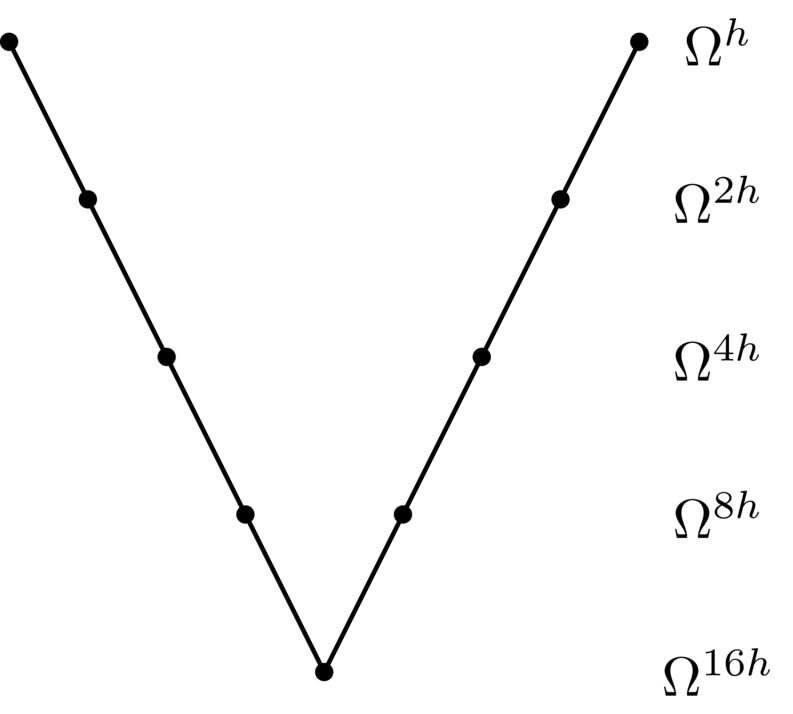
\includegraphics[height=2in]{../Graphics/V-Cycle-Graphic.png}
\end{center}

We can get this cycle by modifying the \texttt{TwoGridScheme} function
above:

    \begin{tcolorbox}[breakable, size=fbox, boxrule=1pt, pad at break*=1mm,colback=cellbackground, colframe=cellborder]
\prompt{In}{incolor}{14}{\boxspacing}
\begin{Verbatim}[commandchars=\\\{\}]
\PY{k}{def} \PY{n+nf}{VCycle}\PY{p}{(}\PY{n}{A\PYZus{}fine}\PY{p}{,} \PY{n}{b}\PY{p}{,} \PY{n}{numPreRelax}\PY{p}{,} \PY{n}{numPostRelax}\PY{p}{,} \PY{n}{coarsest\PYZus{}N}\PY{p}{,} \PY{n}{numiters}\PY{o}{=}\PY{l+m+mi}{1}\PY{p}{,} \PY{n}{x}\PY{o}{=}\PY{k+kc}{None}\PY{p}{)}\PY{p}{:}
    \PY{c+c1}{\PYZsh{} For simplicity, we assume A\PYZus{}fine is (2\PYZca{}n\PYZhy{}1) by (2\PYZca{}n\PYZhy{}1) }
    \PY{c+c1}{\PYZsh{}                       and A\PYZus{}coarse is (2\PYZca{}(n\PYZhy{}1)\PYZhy{}1) by (2\PYZca{}(n\PYZhy{}1)\PYZhy{}1) for some n}
    \PY{c+c1}{\PYZsh{}}
    \PY{c+c1}{\PYZsh{} We will also assume that A is SPD so that we can use CG to solve the coarse system}
    \PY{c+c1}{\PYZsh{}}
    \PY{c+c1}{\PYZsh{} It should be noted that this implementation is not best to use if numiters is not 1}
    \PY{c+c1}{\PYZsh{} since we are not caching the calculated A, I\PYZus{}restrict, I\PYZus{}prolong matrices}
    \PY{c+c1}{\PYZsh{} here we re\PYZhy{}calculate them during each V, doing much extra computation}
    
    \PY{c+c1}{\PYZsh{} Build the restriction and prolongation operators}
    \PY{c+c1}{\PYZsh{} They can be re\PYZhy{}used if we run more than 1 iteration}
    \PY{n}{N} \PY{o}{=} \PY{n}{A\PYZus{}fine}\PY{o}{.}\PY{n}{shape}\PY{p}{[}\PY{l+m+mi}{0}\PY{p}{]}
    \PY{n}{I\PYZus{}Restrict} \PY{o}{=} \PY{n}{BuildFullWeighting}\PY{p}{(}\PY{n}{N}\PY{p}{)}
    \PY{n}{I\PYZus{}Prolong} \PY{o}{=} \PY{l+m+mi}{2}\PY{o}{*}\PY{n}{I\PYZus{}Restrict}\PY{o}{.}\PY{n}{T}
    
    \PY{c+c1}{\PYZsh{} start with the initial guess of zero if one isn\PYZsq{}t given}
    \PY{k}{if} \PY{n}{x} \PY{o+ow}{is} \PY{k+kc}{None}\PY{p}{:}
        \PY{n}{x} \PY{o}{=} \PY{n}{np}\PY{o}{.}\PY{n}{zeros\PYZus{}like}\PY{p}{(}\PY{n}{b}\PY{p}{)}
    
    \PY{c+c1}{\PYZsh{} Calculate the coarse mesh}
    \PY{n}{A\PYZus{}coarse} \PY{o}{=} \PY{n}{I\PYZus{}Restrict}\PY{o}{.}\PY{n}{dot}\PY{p}{(}\PY{n}{A\PYZus{}fine}\PY{o}{.}\PY{n}{dot}\PY{p}{(}\PY{n}{I\PYZus{}Prolong}\PY{p}{)}\PY{p}{)}
    \PY{n}{N\PYZus{}coarse} \PY{o}{=} \PY{n}{A\PYZus{}coarse}\PY{o}{.}\PY{n}{shape}\PY{p}{[}\PY{l+m+mi}{0}\PY{p}{]}
    
    \PY{c+c1}{\PYZsh{} We could run more than once if more accuracy is required}
    \PY{k}{for} \PY{n}{i} \PY{o+ow}{in} \PY{n+nb}{range}\PY{p}{(}\PY{n}{numiters}\PY{p}{)}\PY{p}{:}
        \PY{c+c1}{\PYZsh{} First we relax on the fine grid:}
        \PY{n}{x} \PY{o}{=} \PY{n}{Jacobi}\PY{p}{(}\PY{n}{x}\PY{p}{,} \PY{n}{A\PYZus{}fine}\PY{p}{,} \PY{n}{b}\PY{p}{,} \PY{n}{numiters}\PY{o}{=}\PY{n}{numPreRelax}\PY{p}{)}
    
        \PY{c+c1}{\PYZsh{} Now compute the restricted residual}
        \PY{n}{r\PYZus{}coarse} \PY{o}{=} \PY{n}{mvmult}\PY{p}{(}\PY{n}{I\PYZus{}Restrict}\PY{p}{,} \PY{n}{b} \PY{o}{\PYZhy{}} \PY{n}{mvmult}\PY{p}{(}\PY{n}{A\PYZus{}fine}\PY{p}{,} \PY{n}{x}\PY{p}{)}\PY{p}{)}
    
        \PY{c+c1}{\PYZsh{} If not on the \PYZdq{}bottom of the V\PYZdq{}, we call recursively}
        \PY{k}{if} \PY{n}{N\PYZus{}coarse} \PY{o}{\PYZgt{}} \PY{n}{coarsest\PYZus{}N}\PY{p}{:}
            \PY{c+c1}{\PYZsh{} We start with an initial guess of zero, only 1 iteration to get the V\PYZhy{}Cycle}
            \PY{n}{e\PYZus{}coarse} \PY{o}{=} \PY{n}{VCycle}\PY{p}{(}\PY{n}{A\PYZus{}coarse}\PY{p}{,} \PY{n}{r\PYZus{}coarse}\PY{p}{,} \PY{n}{numPreRelax}\PY{p}{,} \PY{n}{numPostRelax}\PY{p}{,} \PY{n}{coarsest\PYZus{}N}\PY{p}{,} \PY{l+m+mi}{1}\PY{p}{)}
        \PY{k}{else}\PY{p}{:} \PY{c+c1}{\PYZsh{} If on the bottom of the V, we solve the coarsest matrix exactly}
            \PY{p}{(}\PY{n}{conv}\PY{p}{,} \PY{n}{\PYZus{}}\PY{p}{,} \PY{n}{e\PYZus{}coarse}\PY{p}{,} \PY{n}{\PYZus{}}\PY{p}{,} \PY{n}{\PYZus{}}\PY{p}{)} \PY{o}{=} \PY{n}{PCG}\PY{p}{(}\PY{n}{A\PYZus{}coarse}\PY{p}{,} \PY{n}{r\PYZus{}coarse}\PY{p}{,} \PY{n}{maxiter}\PY{o}{=}\PY{l+m+mi}{100000}\PY{p}{)}
            \PY{k}{if} \PY{o+ow}{not} \PY{n}{conv}\PY{p}{:}
                \PY{k}{raise} \PY{n+ne}{RuntimeError}\PY{p}{(}\PY{l+s+s2}{\PYZdq{}}\PY{l+s+s2}{PCG did not converge on the coarse\PYZus{}grid}\PY{l+s+s2}{\PYZdq{}}\PY{p}{)}
                
    
        \PY{c+c1}{\PYZsh{} Correct the fine\PYZhy{}grid x with the prolongated residual}
        \PY{n}{x} \PY{o}{+}\PY{o}{=} \PY{n}{mvmult}\PY{p}{(}\PY{n}{I\PYZus{}Prolong}\PY{p}{,} \PY{n}{e\PYZus{}coarse}\PY{p}{)}
    
        \PY{c+c1}{\PYZsh{} The above Prolongation could be introducing additional high frequency errors}
        \PY{c+c1}{\PYZsh{} So we relax again to get rid of them}
        \PY{n}{x} \PY{o}{=} \PY{n}{Jacobi}\PY{p}{(}\PY{n}{x}\PY{p}{,} \PY{n}{A\PYZus{}fine}\PY{p}{,} \PY{n}{b}\PY{p}{,} \PY{n}{numiters}\PY{o}{=}\PY{n}{numPostRelax}\PY{p}{)}
    
    \PY{k}{return} \PY{n}{x}
\end{Verbatim}
\end{tcolorbox}

    \begin{tcolorbox}[breakable, size=fbox, boxrule=1pt, pad at break*=1mm,colback=cellbackground, colframe=cellborder]
\prompt{In}{incolor}{15}{\boxspacing}
\begin{Verbatim}[commandchars=\\\{\}]
\PY{c+c1}{\PYZsh{} Run VCycle}
\PY{n}{startT} \PY{o}{=} \PY{n}{time}\PY{o}{.}\PY{n}{time}\PY{p}{(}\PY{p}{)}
\PY{n}{x\PYZus{}VCyc} \PY{o}{=} \PY{n}{VCycle}\PY{p}{(}\PY{n}{A\PYZus{}fine}\PY{p}{,} \PY{n}{b}\PY{p}{,} \PY{l+m+mi}{3}\PY{p}{,} \PY{l+m+mi}{3}\PY{p}{,} \PY{l+m+mi}{128}\PY{p}{,} \PY{n}{numiters}\PY{o}{=}\PY{l+m+mi}{1}\PY{p}{)}
\PY{n}{endT} \PY{o}{=} \PY{n}{time}\PY{o}{.}\PY{n}{time}\PY{p}{(}\PY{p}{)}
\PY{n}{relError} \PY{o}{=} \PY{n}{norm}\PY{p}{(}\PY{n}{x\PYZus{}VCyc} \PY{o}{\PYZhy{}} \PY{n}{xTrue}\PY{p}{)}\PY{o}{/}\PY{n}{norm}\PY{p}{(}\PY{n}{xTrue}\PY{p}{)}
\PY{n}{results}\PY{o}{.}\PY{n}{add\PYZus{}row}\PY{p}{(}\PY{p}{[}\PY{l+s+s2}{\PYZdq{}}\PY{l+s+s2}{V\PYZhy{}Cycle (3 pre, 3 post, 127x127 coarse)}\PY{l+s+s2}{\PYZdq{}}\PY{p}{,} \PY{l+m+mi}{1}\PY{p}{,} \PY{n}{relError}\PY{p}{,} \PY{n}{endT}\PY{o}{\PYZhy{}}\PY{n}{startT}\PY{p}{]}\PY{p}{)}

\PY{c+c1}{\PYZsh{} Run VCycle}
\PY{n}{startT} \PY{o}{=} \PY{n}{time}\PY{o}{.}\PY{n}{time}\PY{p}{(}\PY{p}{)}
\PY{n}{x\PYZus{}VCyc} \PY{o}{=} \PY{n}{VCycle}\PY{p}{(}\PY{n}{A\PYZus{}fine}\PY{p}{,} \PY{n}{b}\PY{p}{,} \PY{l+m+mi}{3}\PY{p}{,} \PY{l+m+mi}{3}\PY{p}{,} \PY{l+m+mi}{128}\PY{p}{,} \PY{n}{numiters}\PY{o}{=}\PY{l+m+mi}{3}\PY{p}{)}
\PY{n}{endT} \PY{o}{=} \PY{n}{time}\PY{o}{.}\PY{n}{time}\PY{p}{(}\PY{p}{)}
\PY{n}{relError} \PY{o}{=} \PY{n}{norm}\PY{p}{(}\PY{n}{x\PYZus{}VCyc} \PY{o}{\PYZhy{}} \PY{n}{xTrue}\PY{p}{)}\PY{o}{/}\PY{n}{norm}\PY{p}{(}\PY{n}{xTrue}\PY{p}{)}
\PY{n}{results}\PY{o}{.}\PY{n}{add\PYZus{}row}\PY{p}{(}\PY{p}{[}\PY{l+s+s2}{\PYZdq{}}\PY{l+s+s2}{V\PYZhy{}Cycle (3 pre, 3 post, 127x127 coarse)}\PY{l+s+s2}{\PYZdq{}}\PY{p}{,} \PY{l+m+mi}{3}\PY{p}{,} \PY{n}{relError}\PY{p}{,} \PY{n}{endT}\PY{o}{\PYZhy{}}\PY{n}{startT}\PY{p}{]}\PY{p}{)}

\PY{c+c1}{\PYZsh{} Run VCycle}
\PY{n}{startT} \PY{o}{=} \PY{n}{time}\PY{o}{.}\PY{n}{time}\PY{p}{(}\PY{p}{)}
\PY{n}{x\PYZus{}VCyc} \PY{o}{=} \PY{n}{VCycle}\PY{p}{(}\PY{n}{A\PYZus{}fine}\PY{p}{,} \PY{n}{b}\PY{p}{,} \PY{l+m+mi}{5}\PY{p}{,} \PY{l+m+mi}{5}\PY{p}{,} \PY{l+m+mi}{128}\PY{p}{,} \PY{n}{numiters}\PY{o}{=}\PY{l+m+mi}{1}\PY{p}{)}
\PY{n}{endT} \PY{o}{=} \PY{n}{time}\PY{o}{.}\PY{n}{time}\PY{p}{(}\PY{p}{)}
\PY{n}{relError} \PY{o}{=} \PY{n}{norm}\PY{p}{(}\PY{n}{x\PYZus{}VCyc} \PY{o}{\PYZhy{}} \PY{n}{xTrue}\PY{p}{)}\PY{o}{/}\PY{n}{norm}\PY{p}{(}\PY{n}{xTrue}\PY{p}{)}
\PY{n}{results}\PY{o}{.}\PY{n}{add\PYZus{}row}\PY{p}{(}\PY{p}{[}\PY{l+s+s2}{\PYZdq{}}\PY{l+s+s2}{V\PYZhy{}Cycle (5 pre, 5 post, 127x127 coarse)}\PY{l+s+s2}{\PYZdq{}}\PY{p}{,} \PY{l+m+mi}{1}\PY{p}{,} \PY{n}{relError}\PY{p}{,} \PY{n}{endT}\PY{o}{\PYZhy{}}\PY{n}{startT}\PY{p}{]}\PY{p}{)}

\PY{n}{display}\PY{p}{(}\PY{n}{HTML}\PY{p}{(}\PY{n}{results}\PY{o}{.}\PY{n}{get\PYZus{}html\PYZus{}string}\PY{p}{(}\PY{p}{)}\PY{p}{)}\PY{p}{)}
\end{Verbatim}
\end{tcolorbox}

\begin{center}
\begin{tabular}{lcrr}
  Algorithm & Iter & Rel Error & Time (sec) \\
  \hline
  Jacobi                                  & 100   &  0.87381  & 37.455 \\
  Two Grid (1 pre, 1 post)                & 1	    &  0.29484  &  8.900 \\
  Two Grid (1 pre, 1 post)                & 3	    &  0.23544  & 32.962 \\
  Two Grid (3 pre, 3 post)                & 1	    &  0.23544  & 11.599 \\
  Two Grid (5 pre, 5 post)                & 1     &  0.20961  & 14.517 \\
  CG                                      & 46078 &  0.21183  & 28.235 \\
  V-Cycle (3 pre, 3 post, 127x127 coarse) & 1     &  0.23201  & 4.7490 \\
  V-Cycle (3 pre, 3 post, 127x127 coarse) & 3     &  0.18222  & 13.906 \\
  V-Cycle (5 pre, 5 post, 127x127 coarse) & 1     &  0.20767  & 7.6766
\end{tabular}
\end{center}    

    
    This looks like a good improvement, they are the fastest single run so
far and achieve about the same error as the other runs. During these
runs, I observed that the CPU usage in my multi-core CPU is higher for
the some of the computation and gets lower for the coarser meshes. This
makes sense, those matrices are smaller and hence, take less
computation. This however means that the size of the coarsest grid
might make a difference. If the course grid is too small, the CPU is
under-utilized, and if the coarse grid is too large, CG will take longer
than moving to a coarser grid. Let's see if we can find a more optimal
coarse-grid size.

We run trials of 1 V-Cycle with 5 pre and 5 post relaxations for
differing coarse matrix sizes:

    \begin{tcolorbox}[breakable, size=fbox, boxrule=1pt, pad at break*=1mm,colback=cellbackground, colframe=cellborder]
\prompt{In}{incolor}{16}{\boxspacing}
\begin{Verbatim}[commandchars=\\\{\}]
\PY{n}{coarseGridSize\PYZus{}results} \PY{o}{=} \PY{n}{PrettyTable}\PY{p}{(}\PY{p}{)}
\PY{n}{coarseGridSize\PYZus{}results}\PY{o}{.}\PY{n}{field\PYZus{}names} \PY{o}{=} \PY{p}{[}\PY{l+s+s2}{\PYZdq{}}\PY{l+s+s2}{Coarse Matrix Size}\PY{l+s+s2}{\PYZdq{}}\PY{p}{,} \PY{l+s+s2}{\PYZdq{}}\PY{l+s+s2}{Rel Error}\PY{l+s+s2}{\PYZdq{}}\PY{p}{,} \PY{l+s+s2}{\PYZdq{}}\PY{l+s+s2}{Time (sec)}\PY{l+s+s2}{\PYZdq{}}\PY{p}{]}
\PY{n}{coarseGridSize\PYZus{}results}\PY{o}{.}\PY{n}{align} \PY{o}{=} \PY{l+s+s2}{\PYZdq{}}\PY{l+s+s2}{l}\PY{l+s+s2}{\PYZdq{}}

\PY{n}{relErrors} \PY{o}{=} \PY{n}{np}\PY{o}{.}\PY{n}{ones}\PY{p}{(}\PY{l+m+mi}{14}\PY{p}{)}
\PY{n}{timings} \PY{o}{=} \PY{n}{np}\PY{o}{.}\PY{n}{zeros}\PY{p}{(}\PY{l+m+mi}{14}\PY{p}{)}

\PY{k}{for} \PY{n}{exp} \PY{o+ow}{in} \PY{n+nb}{range}\PY{p}{(}\PY{l+m+mi}{2}\PY{p}{,}\PY{l+m+mi}{16}\PY{p}{)}\PY{p}{:}
    \PY{n}{startT} \PY{o}{=} \PY{n}{time}\PY{o}{.}\PY{n}{time}\PY{p}{(}\PY{p}{)}
    \PY{n}{x\PYZus{}VCyc} \PY{o}{=} \PY{n}{VCycle}\PY{p}{(}\PY{n}{A\PYZus{}fine}\PY{p}{,} \PY{n}{b}\PY{p}{,} \PY{l+m+mi}{5}\PY{p}{,} \PY{l+m+mi}{5}\PY{p}{,} \PY{l+m+mi}{2}\PY{o}{*}\PY{o}{*}\PY{n}{exp}\PY{p}{,} \PY{n}{numiters}\PY{o}{=}\PY{l+m+mi}{1}\PY{p}{)}
    \PY{n}{endT} \PY{o}{=} \PY{n}{time}\PY{o}{.}\PY{n}{time}\PY{p}{(}\PY{p}{)}
    \PY{n}{relErrors}\PY{p}{[}\PY{n}{exp}\PY{o}{\PYZhy{}}\PY{l+m+mi}{2}\PY{p}{]} \PY{o}{=} \PY{n}{norm}\PY{p}{(}\PY{n}{x\PYZus{}VCyc} \PY{o}{\PYZhy{}} \PY{n}{xTrue}\PY{p}{)}\PY{o}{/}\PY{n}{norm}\PY{p}{(}\PY{n}{xTrue}\PY{p}{)}
    \PY{n}{timings}\PY{p}{[}\PY{n}{exp}\PY{o}{\PYZhy{}}\PY{l+m+mi}{2}\PY{p}{]} \PY{o}{=} \PY{n}{endT}\PY{o}{\PYZhy{}}\PY{n}{startT}
    \PY{n}{coarseGridSize\PYZus{}results}\PY{o}{.}\PY{n}{add\PYZus{}row}\PY{p}{(}\PY{p}{[}\PY{l+s+sa}{f}\PY{l+s+s1}{\PYZsq{}}\PY{l+s+si}{\PYZob{}}\PY{l+m+mi}{2}\PY{o}{*}\PY{o}{*}\PY{n}{exp} \PY{o}{\PYZhy{}} \PY{l+m+mi}{1}\PY{l+s+si}{\PYZcb{}}\PY{l+s+s1}{x}\PY{l+s+si}{\PYZob{}}\PY{l+m+mi}{2}\PY{o}{*}\PY{o}{*}\PY{n}{exp}\PY{o}{\PYZhy{}}\PY{l+m+mi}{1}\PY{l+s+si}{\PYZcb{}}\PY{l+s+s1}{\PYZsq{}}\PY{p}{,} \PY{n}{relErrors}\PY{p}{[}\PY{n}{exp}\PY{o}{\PYZhy{}}\PY{l+m+mi}{2}\PY{p}{]}\PY{p}{,} \PY{n}{timings}\PY{p}{[}\PY{n}{exp}\PY{o}{\PYZhy{}}\PY{l+m+mi}{2}\PY{p}{]}\PY{p}{]}\PY{p}{)}
    
\PY{n}{display}\PY{p}{(}\PY{n}{HTML}\PY{p}{(}\PY{n}{coarseGridSize\PYZus{}results}\PY{o}{.}\PY{n}{get\PYZus{}html\PYZus{}string}\PY{p}{(}\PY{p}{)}\PY{p}{)}\PY{p}{)}
\end{Verbatim}
\end{tcolorbox}

\begin{center}    
  \begin{tabular}{crr}
    Coarse Matrix Size & Rel Error & Time (sec) \\
    \hline
    3x3         & 0.20863 & 7.64522 \\
    7x7         & 0.20801 & 7.70789 \\
    15x15       & 0.20784 & 7.62153 \\
    31x31       & 0.20774 & 7.64096 \\
    63x63       & 0.20768 & 7.68061 \\
    127x127     & 0.20767 & 7.65519 \\
    255x255     & 0.20766 & 7.82747 \\
    511x511     & 0.20767 & 7.94081 \\
    1023x1023   & 0.20770 & 8.07504 \\
    2047x2047   & 0.20777 & 7.64995 \\
    4095x4095   & 0.20790 & 7.38173 \\
    8191x8191   & 0.20816 & 7.14767 \\
    16383x16383 & 0.20868 & 8.89681 \\
    32767x32767 & 0.20961 & 14.0686
  \end{tabular}
\end{center}

    
    It appears that a \(8191\times 8191\) matrix is the most efficient
coarse grid size for this computer. Any larger and the CG method takes
too long, either due to cache size, number of cache misses, or simply
the number of iterations CG needs to converge for the coarse problem
(due to the increased condition number). Let's add this run to our table
to see all the results together:

    \begin{tcolorbox}[breakable, size=fbox, boxrule=1pt, pad at break*=1mm,colback=cellbackground, colframe=cellborder]
\prompt{In}{incolor}{17}{\boxspacing}
\begin{Verbatim}[commandchars=\\\{\}]
\PY{n}{results}\PY{o}{.}\PY{n}{add\PYZus{}row}\PY{p}{(}\PY{p}{[}\PY{l+s+s2}{\PYZdq{}}\PY{l+s+s2}{V\PYZhy{}Cycle (5 pre, 5 post, 8191x8191 coarse)}\PY{l+s+s2}{\PYZdq{}}\PY{p}{,} \PY{l+m+mi}{1}\PY{p}{,} \PY{n}{relErrors}\PY{p}{[}\PY{l+m+mi}{11}\PY{p}{]}\PY{p}{,} \PY{n}{timings}\PY{p}{[}\PY{l+m+mi}{11}\PY{p}{]}\PY{p}{]}\PY{p}{)}

\PY{n}{display}\PY{p}{(}\PY{n}{HTML}\PY{p}{(}\PY{n}{results}\PY{o}{.}\PY{n}{get\PYZus{}html\PYZus{}string}\PY{p}{(}\PY{p}{)}\PY{p}{)}\PY{p}{)}
\end{Verbatim}
\end{tcolorbox}

\begin{center}    
\begin{tabular}{lcrr}
  Algorithm & Iter & Rel Error & Time (sec) \\
  \hline
  Jacobi                                    & 100   &  0.87381  & 37.455 \\
  Two Grid (1 pre, 1 post)                  & 1	    &  0.29484  &  8.900 \\
  Two Grid (1 pre, 1 post)                  & 3	    &  0.23544  & 32.962 \\
  Two Grid (3 pre, 3 post)                  & 1	    &  0.23544  & 11.599 \\
  Two Grid (5 pre, 5 post)                  & 1     &  0.20961  & 14.517 \\
  CG                                        & 46078 &  0.21183  & 28.235 \\
  V-Cycle (3 pre, 3 post, 127x127 coarse)   & 1     &  0.23201  & 4.7490 \\
  V-Cycle (3 pre, 3 post, 127x127 coarse)   & 3     &  0.18222  & 13.906 \\
  V-Cycle (5 pre, 5 post, 127x127 coarse)   & 1     &  0.20767  & 7.6766 \\
  V-Cycle (5 pre, 5 post, 8191x8191 coarse) & 1     &  0.20816  & 7.1476
\end{tabular}
\end{center}

    
    Finally, let's run some extra iterations to see what the convergence
looks like. Since the code below interrupts the V-Cycle function after
every V-Cycle, we are doing extra work and so the timings are not
representative, hence we won't calculate them.

    \begin{tcolorbox}[breakable, size=fbox, boxrule=1pt, pad at break*=1mm,colback=cellbackground, colframe=cellborder]
\prompt{In}{incolor}{18}{\boxspacing}
\begin{Verbatim}[commandchars=\\\{\}]
\PY{n}{maxIters} \PY{o}{=} \PY{l+m+mi}{30}
\PY{n}{coarseGridSize} \PY{o}{=} \PY{l+m+mi}{2}\PY{o}{*}\PY{o}{*}\PY{l+m+mi}{13}
\PY{n}{numRelax} \PY{o}{=} \PY{l+m+mi}{5}

\PY{c+c1}{\PYZsh{} container to hold the errors}
\PY{n}{relError} \PY{o}{=} \PY{n}{np}\PY{o}{.}\PY{n}{ones}\PY{p}{(}\PY{n}{maxIters}\PY{o}{+}\PY{l+m+mi}{1}\PY{p}{)}

\PY{c+c1}{\PYZsh{} Provide an initial guess}
\PY{n}{x\PYZus{}VCyc} \PY{o}{=} \PY{n}{np}\PY{o}{.}\PY{n}{zeros\PYZus{}like}\PY{p}{(}\PY{n}{b}\PY{p}{)}

\PY{k}{for} \PY{n}{i} \PY{o+ow}{in} \PY{n+nb}{range}\PY{p}{(}\PY{l+m+mi}{1}\PY{p}{,}\PY{n}{maxIters}\PY{o}{+}\PY{l+m+mi}{1}\PY{p}{)}\PY{p}{:}
    \PY{n}{x\PYZus{}VCyc} \PY{o}{=} \PY{n}{VCycle}\PY{p}{(}\PY{n}{A\PYZus{}fine}\PY{p}{,} \PY{n}{b}\PY{p}{,} \PY{n}{numRelax}\PY{p}{,} \PY{n}{numRelax}\PY{p}{,} \PY{n}{coarseGridSize}\PY{p}{,} \PY{n}{numiters}\PY{o}{=}\PY{l+m+mi}{1}\PY{p}{,} \PY{n}{x}\PY{o}{=}\PY{n}{x\PYZus{}VCyc}\PY{p}{)}
    \PY{n}{relError}\PY{p}{[}\PY{n}{i}\PY{p}{]} \PY{o}{=} \PY{n}{norm}\PY{p}{(}\PY{n}{x\PYZus{}VCyc} \PY{o}{\PYZhy{}} \PY{n}{xTrue}\PY{p}{)}\PY{o}{/}\PY{n}{norm}\PY{p}{(}\PY{n}{xTrue}\PY{p}{)}

\PY{n}{plt}\PY{o}{.}\PY{n}{plot}\PY{p}{(}\PY{n}{relError}\PY{p}{)}
\end{Verbatim}
\end{tcolorbox}

            \begin{tcolorbox}[breakable, size=fbox, boxrule=.5pt, pad at break*=1mm, opacityfill=0]
\prompt{Out}{outcolor}{18}{\boxspacing}
\begin{Verbatim}[commandchars=\\\{\}]
[<matplotlib.lines.Line2D at 0x7f39eaaf60a0>]
\end{Verbatim}
\end{tcolorbox}
        
    \begin{center}
    \adjustimage{max size={0.9\linewidth}{0.9\paperheight}}{output_45_1.png}
    \end{center}
    { \hspace*{\fill} \\}
    
    Notice the large decrease in error from the first iteration (80\%
reduction). This is one of the primary reasons why one iteration of
multigrid is widely used as a preconditioner.

    \hypertarget{other-multigrid-cycles}{%
\section{Other Multigrid Cycles}\label{other-multigrid-cycles}}

While the V-Cycle is the most popular, there are other proposed cycles
as well. One possible extension is to recursively run two consecutive
V-Cycles:
\begin{center}
  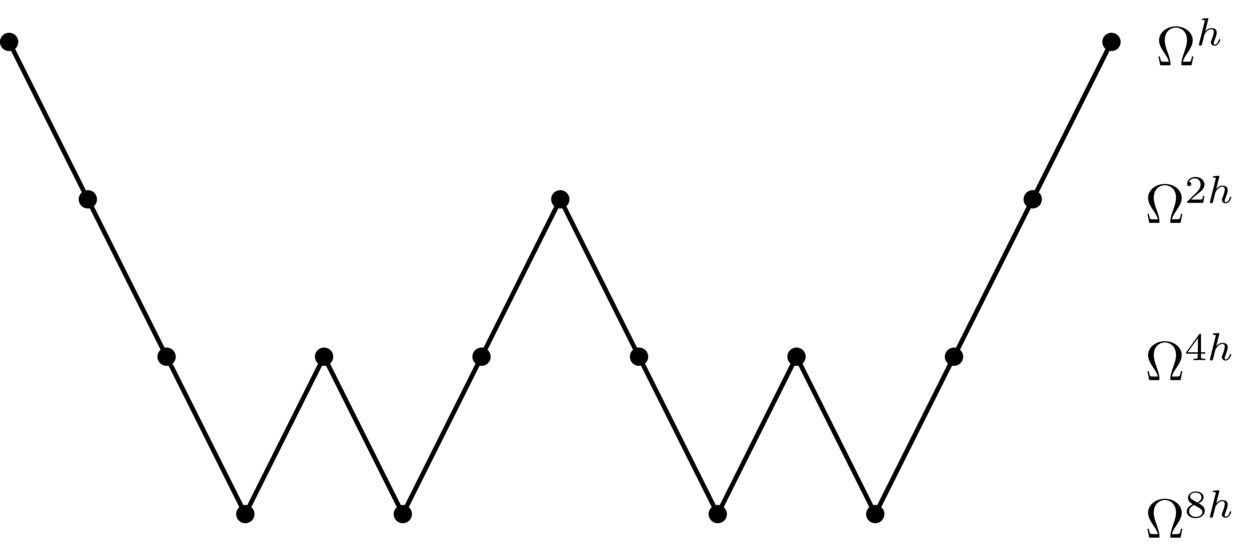
\includegraphics[height=1.8in]{../Graphics/W-Cycle-Graphic.png}
\end{center}
This is typically called a \textbf{W-Cycle}. You can of course extend
this to running more than 2 consecutive V-Cycles, Briggs's book calls
these \textbf{\(\mu\)-Cycles} (where \(\mu\) refers to the number of
consecutive V-Cycles completed recursively).

Finally, there is the \textbf{Full Multigrid Cycle}:
\begin{center}
  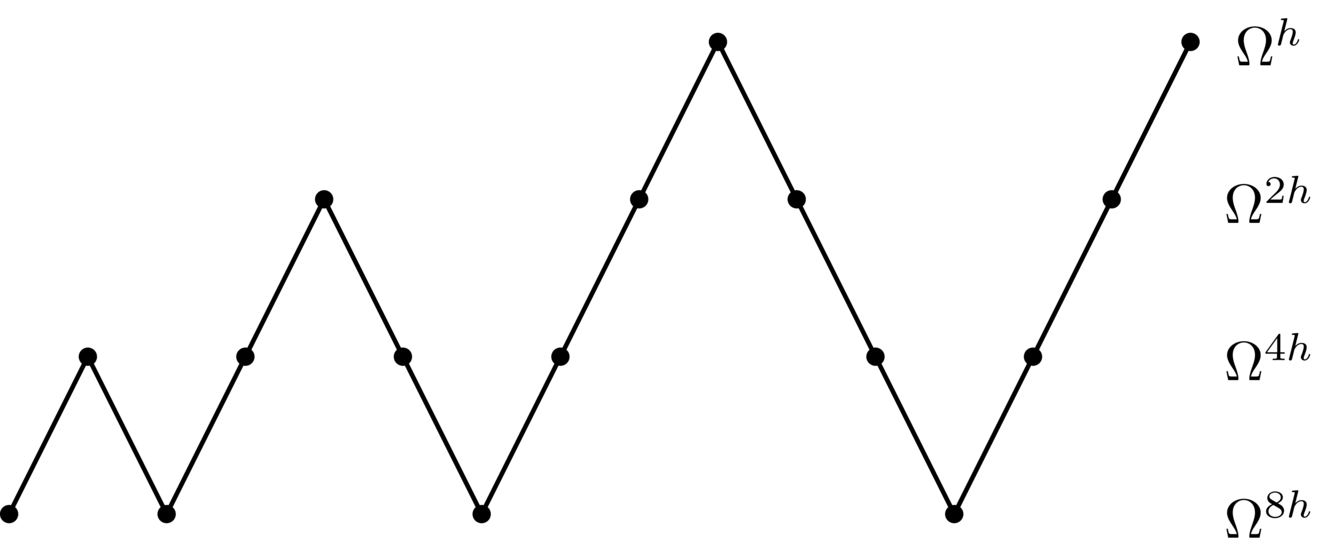
\includegraphics[height=1.8in]{../Graphics/FMV-Cycle-Graphic.png}
\end{center}
The idea behind the full multigrid cycle is to first solve on the coarse
grid, getting a good starting guess for the next finer grid. Then run a
V-Cycle on that grid to get a good starting point for the next finer
grid, and continue that process until the finest grid is reached.

    \hypertarget{tuning-multigrid}{%
\section{Tuning Multigrid}\label{tuning-multigrid}}

There are several ``knobs to turn'' to tune Multigrid Methods:
\begin{itemize}
\item Several different relaxation schemes have been shown to be effective: weighted
Jacobi, Red-Black Jacobi, Gauss-Seidel, Red-Black Gauss Seidel, SOR,
Block Jacobi, Block Gauss-Seidel 
\item Method for solving the coarsest grid problem can be chosen 
\item The number of relaxations can have some effect in the convergence of the
  method, typically 3-5 are used 
\item Which type of cycle to use: the most common is the V-Cycle, but the W and Full
Multigrid Cycle are also common, \(\mu\)-cycles with \(\mu \geq 3\) are
rarely seen
\end{itemize}

    \hypertarget{cons-of-multigrid}{%
\section{Cons of Multigrid}\label{cons-of-multigrid}}

While the multigrid method has been shown to be effective in terms of
computational time, it does cost more in terms of memory. This is due to
the fact that all grids need to be in storage at once. The cost here is
mitigated, however, since the dimensions of the coarse matrices decreases
exponentially.

Another negative aspect of multrigrid is the fact that it is not as
effective on smaller matrices. For example, straight CG is often faster
than multigrid for smaller matrix sizes, where CG does not have to
complete as many iterations.

    \hypertarget{algebraic-multigrid}{%
\section{Algebraic Multigrid}\label{algebraic-multigrid}}

While geometric multigrid is useful for gaining intuition into multigrid
methods, it's not often used in practice. It's tougher to design the
restriction and prolongation operators for non-uniform meshes where the
number of bordering nodes is variable. It's also less useful for systems
with more than one state variable, since only the physical dimensions
can be made coarser. Instead, we will use the same idea to develop a
multigrid method that doesn't explicitly depend on the mesh, but instead
depends on the coefficient matrix.

If we look at our matrix \[
A = \frac{1}{h^2}
\begin{bmatrix}
2  & -1 &        &        &        &   \\
-1 &  2 & -1     &        &        &   \\
   & -1 &  2     &     -1 &        &   \\
   &    & \ddots & \ddots & \ddots &   \\
   &    &        &     -1 &      2 & -1 \\
   &    &        &        &     -1 &  2
\end{bmatrix}
\] we can interpret it in the following way: an entry's magnitude in the
matrix corresponds to its level of contribution in calculating the
element on the diagonal. For example, row 2 has \(-1/h^2\), \(2/h^2\),
and \(-1/h^2\) in the first three columns. This signifies that only
\(x_1, x_2, x_3\) directly contribute to the node \(x_2\), with the
value \(x_2\) contributing more than \(x_1\) and \(x_3\). In algebraic
multigrid, we use this idea of ``significance'' to determine which
unknowns can be ``merged'' to obtain a coarse matrix. This process will
also create prolongation and restriction operators which only depend on
the coefficient matrix and not on the geometric structure of the
physical problem. Algebraic multigrid can therefore be programmed in a
more general way and can more easily extended to more problems. This
property also contributes to its usefulness as a preconditioner since it
takes less setup and quickly gives modest accuracy.


    % Add a bibliography block to the postdoc
    
    
    
\end{document}
